\documentclass[a4paper,11pt,openany,extrafontsizes]{memoir}

\usepackage{fontspec}

\setmainfont[Numbers=OldStyle]{Linux Libertine O}
\setsansfont[Numbers=OldStyle]{Linux Biolinum O}
\setmonofont[Scale=0.83]{Inconsolata}

\usepackage{polyglossia}
\setdefaultlanguage[variant=british]{english}

\usepackage{lipsum}

\usepackage{graphicx}
\usepackage[dvipsnames]{xcolor}
\usepackage{wrapfig}
\usepackage{subcaption}
\usepackage{lettrine}

\usepackage{amssymb, amsmath}
\usepackage{amsthm}

\theoremstyle{plain}
\newtheorem{thm}{Theorem}[chapter]
\newtheorem{lem}[thm]{Lemma}
\newtheorem{cor}[thm]{Corollary}
\newtheorem{prop}[thm]{Proposition}
\theoremstyle{definition}
\newtheorem{defn}{Definition}[chapter]
\newtheorem{expl}{Example}[chapter]
\theoremstyle{remark}
\newtheorem*{rem}{Remark}
\newtheorem*{note}{Note}
\newtheorem*{notation}{Notation}

\usepackage{pdfpages}

\usepackage{microtype}

%% Propriétés du document PDF
\usepackage[unicode,colorlinks=true]{hyperref}

\hypersetup{
  pdfauthor={Dimitri Lozeve},
  pdftitle={Topological Data Analysis of Temporal Networks},
  pdfsubject={A dissertation submitted un partial fulfilment of the degree of Master of Science in Applied Statistics},
  pdfkeywords={dissertation,stats,msc,tda,networks},
  pdfpagemode=UseOutlines,
  pdfpagelayout=TwoColumnRight,
  linkcolor=MidnightBlue,
  filecolor=MidnightBlue,
  urlcolor=MidnightBlue,
  citecolor=Green
}

%% Pour la classe memoir /!\

%% Marges
\setlrmarginsandblock{3cm}{3cm}{*}
\setulmarginsandblock{3cm}{3cm}{*}
\checkandfixthelayout%

%% Numérotation des divisions logiques
\setsecnumdepth{subsection}
\maxsecnumdepth{subsection}

%% Profondeur de la ToC
\settocdepth{subsection}
\maxtocdepth{subsection}

%% Style des titres des divisions logiques
\setsecheadstyle{\Large\scshape}
\setsubsecheadstyle{\large\scshape}

%% Abstract
\abstractintoc%
\renewcommand{\abstractnamefont}{\normalfont\large\scshape}
\renewcommand{\abstracttextfont}{\normalfont\normalsize}

%% épigraphes
\setlength{\epigraphwidth}{0.5\textwidth}
\epigraphtextposition{flushleftright}

%% Couleurs
%\definecolor{purpletouch}{RGB}{103,30,117}
\definecolor{bleux}{RGB}{0,62,92}

\author{Dimitri Lozeve}
\date{September 2018}
\title{Topological Data Analysis of Temporal Networks}







%%% Local Variables:
%%% mode: latex
%%% TeX-master: "dissertation"
%%% End:


\begin{document}

\pagestyle{plain}
\tightlists%

\begin{titlingpage}
  \begin{center}
    \vspace{1cm}
    \textsf{\Huge{University of Oxford}}\\
    \vspace{1cm}
    
\includegraphics{branding/beltcrest.png}\\
    \vspace{2cm}
    \Huge{\thetitle}\\
    \vspace{2cm}
    \large{by\\[14pt]\theauthor\\[8pt]St Catherine's College}
    \vfill
    %% Inkscape L-system
    %% [C]++[C]++[C]++[C]++[C]
    %% B=DA++EA----CA[-DA----BA]++;C=+DA--EA[---BA--CA]+;D=-BA++CA[+++DA++EA]-;E=--DA++++BA[+EA++++CA]--CA;A=
    % \begin{tikzpicture}
    %   \pgfdeclarelindenmayersystem{Penrose}{
    %     \symbol{M}{\pgflsystemdrawforward}
    %     \symbol{N}{\pgflsystemdrawforward}
    %     \symbol{O}{\pgflsystemdrawforward}
    %     \symbol{P}{\pgflsystemdrawforward}
    %     \symbol{A}{\pgflsystemdrawforward}
    %     \symbol{+}{\pgflsystemturnright}
    %     \symbol{-}{\pgflsystemturnleft}
    %     \rule{M->OA++PA----NA[-OA----MA]++}
    %     \rule{N->+OA--PA[---MA--NA]+}
    %     \rule{O->-MA++NA[+++OA++PA]-}
    %     \rule{P->--OA++++MA[+PA++++NA]--NA}
    %     \rule{A->}
    %   }
    %   \draw[lindenmayer system={Penrose, axiom=[N]++[N]++[N]++[N]++[N],
    %     order=2, angle=36, step=4pt}]
    %   lindenmayer system;
    % \end{tikzpicture}
    % \vspace{2.2cm}
    \vfill
    \large{A dissertation submitted in partial fulfilment of the requirements for the degree of\\
      Master of Science in Statistical Science}\\
    \vspace{.5cm}
    \large{\emph{Department of Statistics,\\ 24--29 St Giles, Oxford, OX1 3LB}}\\
    \vspace{1cm} \large{\thedate}
  \end{center}
\end{titlingpage}

%\chapterstyle{hangnum}
%\chapterstyle{ell}
%\chapterstyle{southall}
\chapterstyle{wilsondob}

\frontmatter

\cleardoublepage%

\vspace*{3cm}
\begin{abstract}
  Temporal networks are a mathematical model to represent interactions
  evolving over time. As such, they have a multitude of applications,
  from biology to physics to social networks. The study of dynamics on
  networks is an emerging field, with many challenges in modelling and
  data analysis.

  An important issue is to uncover meaningful temporal structure in a
  network. We focus on the problem of periodicity detection in
  temporal networks, by partitioning the time range of the network and
  clustering the resulting subnetworks.

  For this, we leverage methods from the field of topological data
  analysis and persistent homology. These methods have begun to be
  employed with static graphs in order to provide a summary of
  topological features, but applications to temporal networks have
  never been studied in detail.

  We cluster temporal networks by computing the evolution of
  topological features over time. Applying persistent homology to
  temporal networks and comparing various approaches has never been
  done before, and we examine their performance side-by-side with a
  simple clustering algorithm. Using a generative model, we show that
  persistent homology is able to detect periodicity in the topological
  structure of a network.

  We define two types of topological features, with and without
  aggregating the temporal networks, and multiple ways of embedding
  them in a feature space suitable for machine-learning
  applications. In particular, we examine the theoretical guarantees
  and empirical performance of kernels defined on topological
  features.

  Topological insights prove to be useful in statistical learning
  applications. Combined with the recent advances in network science,
  they lead to a deeper understanding of the structure of temporal
  networks.
\end{abstract}
\vspace*{\fill}

\cleardoublepage%

\chapter{Acknowledgements}%
\label{cha:acknowledgements}

I would like to thank my supervisors, Dr Heather Harrington, Dr Renaud
Lambiotte, and Dr Mason Porter, from the Mathematical Institute, for
their continuous support and guidance from the very beginning. They
have allowed me to pursue my interests in networks and topological
data analysis while providing me with resources, ideas, and
motivation. They remained available to answer my questions and listen
to my ideas, and provided invaluable feedback at every stage of the
project.

I would also like to thank Dr Steve Oudot from École polytechnique,
who was the first to introduce me to the field of topological data
analysis, which led me to the original idea for the project. He was
also very helpful during the project, giving me advice and updates on
recent advances in persistent homology.

I also want to acknowledge the students and staff of the Department of
Statistics and St Catherine's college, who always provided a
stimulating work environment, along with excellent discussions.

Finally, my thanks go to my family and friends for their interest in
my project, because trying to explain it to people not acquainted with
the topic was, and remains, the best way to clarify my ideas and
organise my thoughts.

\cleardoublepage%

\tableofcontents

\clearpage

\listoffigures

\begingroup
\let\clearpage\relax
\listofalgorithms%
\addcontentsline{toc}{chapter}{List of Algorithms}
\endgroup

\clearpage

\mainmatter%

\chapter{Introduction}%
\label{cha:introduction}

\section{Temporal networks analysis}%
\label{sec:temp-netw-analys}

Networks are one of the most important mathematical concepts developed
in the last few centuries. They allow the representation of
interconnected data and complex systems. As such, the concept has been
applied to wide variety of problems, in biology and neuroscience,
physics, computer networks, and social science. In this context,
network science has emerged as a discipline of its own, combining
ideas and challenges from multiple fields of
study~\cite{newman_networks:_2010}.

\captionsetup[figure]{labelformat=empty}

\begin{wrapfigure}[15]{R}[.3cm]{.3\linewidth}
  \centering
  \vspace{-15pt}
  \SetCoordinates[yAngle=45]
  \begin{tikzpicture}[multilayer=3d]
    \SetLayerDistance{-2}
    \Plane[x=.5,y=.5,width=3,height=3,style={thin,dashed},layer=1]
    \Plane[x=.5,y=.5,width=3,height=3,style={thin,dashed},layer=2]
    \Plane[x=.5,y=.5,width=3,height=3,style={thin,dashed},layer=3]
    \begin{Layer}[layer=1]
      \node at (.5,.5)[below right] {Time $t_1$};
    \end{Layer}
    \begin{Layer}[layer=2]
      \node at (.5,.5)[below right] {Time $t_2$};
    \end{Layer}
    \begin{Layer}[layer=3]
      \node at (.5,.5)[below right] {Time $t_3$};
    \end{Layer}

    \Vertex[x=1.408,y=1.635,size=0.3,color=blue,opacity=0.7,layer=1]{0_1}
    \Vertex[x=1.089,y=2.415,size=0.3,color=blue,opacity=0.7,layer=1]{1_1}
    \Vertex[x=2.021,y=1.976,size=0.3,color=blue,opacity=0.7,layer=1]{2_1}
    \Vertex[x=1.984,y=3.000,size=0.3,color=blue,opacity=0.7,layer=1]{3_1}
    \Vertex[x=2.576,y=2.398,size=0.3,color=blue,opacity=0.7,layer=1]{4_1}
    \Vertex[x=2.911,y=1.593,size=0.3,color=blue,opacity=0.7,layer=1]{5_1}
    \Vertex[x=1.994,y=1.000,size=0.3,color=blue,opacity=0.7,layer=1]{6_1}
    \Edge[](1_1)(3_1)
    \Edge[](3_1)(4_1)
    \Edge[](3_1)(4_1)
    \Edge[](0_1)(5_1)
    \Edge[](0_1)(5_1)
    \Edge[](2_1)(5_1)
    \Edge[](4_1)(5_1)
    \Edge[](0_1)(6_1)
    \Edge[](1_1)(6_1)
    \Edge[](5_1)(6_1)

    \Vertex[x=1.408,y=1.635,size=0.3,color=blue,opacity=0.7,layer=2]{0_2}
    \Vertex[x=1.089,y=2.415,size=0.3,color=blue,opacity=0.7,layer=2]{1_2}
    \Vertex[x=2.021,y=1.976,size=0.3,color=blue,opacity=0.7,layer=2]{2_2}
    \Vertex[x=1.984,y=3.000,size=0.3,color=blue,opacity=0.7,layer=2]{3_2}
    \Vertex[x=2.576,y=2.398,size=0.3,color=blue,opacity=0.7,layer=2]{4_2}
    \Vertex[x=2.911,y=1.593,size=0.3,color=blue,opacity=0.7,layer=2]{5_2}
    \Vertex[x=1.994,y=1.000,size=0.3,color=blue,opacity=0.7,layer=2]{6_2}
    \Edge[](1_2)(2_2)
    \Edge[](0_2)(3_2)
    \Edge[](2_2)(4_2)
    \Edge[](2_2)(6_2)

    \Vertex[x=1.408,y=1.635,size=0.3,color=blue,opacity=0.7,layer=3]{0_3}
    \Vertex[x=1.089,y=2.415,size=0.3,color=blue,opacity=0.7,layer=3]{1_3}
    \Vertex[x=2.021,y=1.976,size=0.3,color=blue,opacity=0.7,layer=3]{2_3}
    \Vertex[x=1.984,y=3.000,size=0.3,color=blue,opacity=0.7,layer=3]{3_3}
    \Vertex[x=2.576,y=2.398,size=0.3,color=blue,opacity=0.7,layer=3]{4_3}
    \Vertex[x=2.911,y=1.593,size=0.3,color=blue,opacity=0.7,layer=3]{5_3}
    \Vertex[x=1.994,y=1.000,size=0.3,color=blue,opacity=0.7,layer=3]{6_3}
    \Edge[](0_3)(2_3)
    \Edge[](0_3)(2_3)
    \Edge[](1_3)(4_3)
    \Edge[](2_3)(5_3)
    \Edge[](4_3)(5_3)
    \Edge[](0_3)(6_3)
    \Edge[](2_3)(6_3)
    \Edge[](4_3)(6_3)
  \end{tikzpicture}
  \caption[Multilayer network.]{}%
  \label{fig:multilayer}
\end{wrapfigure}

\captionsetup[figure]{labelformat=default}

An emerging trend in network science is the study of dynamics on
networks~\cite{holme_temporal_2012, holme_modern_2015,
  porter_dynamical_2014}. Real-world systems, such as brains or social
groups, tend to evolve over time, and these changing networks have
given birth to the new field of network dynamics, where edges can
reconfigure over time. Mathematical modelling of temporal connectivity
patterns remain a difficult
problem~\cite{bassett_network_2017}. Recent advances in applied
mathematics have led to may concurrent representations, multilayer
networks~\cite{kivela_multilayer_2014} being one of the most
important.

Temporal networks bring new challenges in size, shape, and complexity
of data analysis, but also new opportunities with the development of
new empirical methods and theoretical advances. One of these advances
is the development of generative models that can be used to infer the
dynamic mechanisms taking place in real-world
systems~\cite{bazzi_generative_2016, gauvin_randomized_2018,
  petri_simplicial_2018}.

Moreover, network theory naturally exposes many links with
topology. The purpose of networks lies in the representation of
\emph{structure}, while topology is the study of spaces and
\emph{connectedness}. As topological methods gain traction in data
science and statistical learning, they are also applied to more
complex data representations, including
networks~\cite{horak_persistent_2009, petri_topological_2013,
  stolz_persistent_2017}. Topological features naturally complement
more traditional network statistics by focusing on mesoscale
structure.


\section{Related work}%
\label{sec:related-work}

Topological data analysis (TDA) is a recent
field~\cite{carlsson_topology_2009}. It was originally focused on
point cloud data, with only a recent shift towards network
data~\cite{horak_persistent_2009}. Various methods have been
developed, the main one being the weight-rank clique filtration
(WRCF)~\cite{petri_topological_2013}. Other examples of application of
TDA to networks using WRCF can be found in~\cite{otter_roadmap_2017}.

There has also been attempts to map the nodes of a network to points
in a metric space. For instance, the shortest-path distance between
nodes can be used to compute pairwise distances in the network. Note
that for this method to work properly, the network has to be
connected. Many methods can be used to build a simplicial complex from
a directed or undirected network~\cite{jonsson_simplicial_2008,
  horak_persistent_2009}.

The main starting point for this project was the introduction of TDA
for the study of temporal networks
in~\cite{price-wright_topological_2015}. In this dissertation,
topological methods are introduced to classify temporal networks
randomly generated by different models. The objective of this study
was to uncover the temporal structure of a network in order to inform
its partitioning into ``snapshots''. Different methods to partition a
network were compared for the first time, and topological features
appeared to be relevant for distinguishing various temporal
distributions.

Finally, there has been an increasing interest in using the
topological structure of a dataset as an additional source of
information for a statistical learning model. This has led to the
development of topological descriptors suitable for use in various
learning contexts. Previous work on vectorizations and kernels on
topological features will be useful in the analysis of the structure
of temporal networks.

\section{Contributions}%
\label{sec:contributions}

The main contributions of this work are threefold:
\begin{itemize}
\item We make an attempt at temporal partitioning networks and
  clustering the subnetworks, with immediate application for detecting
  periodicity. Sliding windows and persistent homology have been used
  in the context of periodicity detection
  before~\cite{perea_sw1pers:_2015, perea_sliding_2017}, but never in
  the context of temporal networks.
\item In general, topological methods have never been thoroughly
  studied on temporal network data. The work
  in~\cite{price-wright_topological_2015} is the first to introduce
  the topic, but computation was limited due to the lack of available
  libraries. Here, we introduce recent (from the last 2--3 years)
  state-of-the-art topological methods and adapt them to temporal
  networks.
\item Various methods to use topological features in a statistical
  learning context and their trade-offs are exposed. The mathematical
  background and practical considerations are leveraged to compare
  them in the context of machine learning.
\item Finally, different topological approaches are compared. There
  are different ways to build a simplicial filtration on a network,
  and different manners of measuring distances between the outputs of
  persistent homology in the context of machine learning. These
  different methods are compared here with the objective of
  periodicity detection in temporal networks.
\end{itemize}


\chapter{Graphs and Temporal Networks}%
\label{cha:temporal-networks}

\section{Definition and basic properties}%
\label{sec:defin-basic-prop}

In this section, we introduce the notion of temporal networks (or
temporal graphs). This is a complex notion, with many concurrent
definitions and interpretations.

After clarifying the notations, we restate the standard definition of
a non-temporal graph.

\begin{notation}
  \begin{itemize}
  \item $\mathbb{N}$ is the set of non-negative natural numbers
    $0,1,2,\ldots$ 
  \item $\mathbb{N}^*$ is the set of positive integers $1,2,\ldots$
  \item $\mathbb{R}$ is the set of real numbers.
    $\mathbb{R}_+ = \{x\in\mathbb{R} \;|\; x\geq 0\}$, and
    $\mathbb{R}_+^* = \{x\in\mathbb{R} \;|\; x>0\}$.
\end{itemize}
\end{notation}

\begin{defn}[Graph]
  A \emph{graph} is a couple $G = (V, E)$, where $V$ is a set of
  \emph{nodes} (or \emph{vertices}), and $E \subseteq V\times V$ is a
  set of \emph{edges}. A \emph{weighted graph} is defined by
  $G = (V, E, w)$, where $w : E\mapsto \mathbb{R}_+^*$ is called the
  \emph{weight function}.
\end{defn}

We also define some basic concepts that we will need later to build
simplicial complexes on graphs.

\begin{defn}[Clique]
  A \emph{clique} is a set of nodes where each pair is adjacent. That
  is, a clique $C$ of a graph $G = (V,E)$ is a subset of $V$ such that
  for all $i,j\in C, i \neq j \implies (i,j)\in E$. A clique is said
  to be \emph{maximal} if it cannot be augmented by any node, such
  that the resulting set of nodes is itself a clique.
\end{defn}

Temporal networks can be defined in the more general framework of
\emph{multilayer networks}~\cite{kivela_multilayer_2014}. However,
this definition is much too general for our simple applications, and
we restrict ourselves to edge-centric time-varying
graphs~\cite{casteigts_time-varying_2012}. In this model, the set of
nodes is fixed, but edges can appear or disappear at different times.

In this study, we restrict ourselves to discrete time stamps. Each
interaction is taken to be instantaneous.

\begin{defn}[Temporal network]\label{defn:temp-net}
  A \emph{temporal network} is a tuple
  $G = (V, E, \mathcal{T}, \rho)$, where:
  \begin{itemize}
  \item $V$ is a set of nodes,
  \item $E\subseteq V\times V$ is a set of edges,
  \item $\mathbb{T}$ is the \emph{temporal domain} (often taken as
    $\mathbb{N}$ or any other countable set), and
    $\mathcal{T}\subseteq\mathbb{T}$ is the \emph{lifetime} of the
    network,
  \item $\rho: E\times\mathcal{T}\mapsto\{0,1\}$ is the \emph{presence
      function}, which determines whether an edge is present in the
    network at each time stamp.
  \end{itemize}
  The \emph{available times} of an edge are the set
  $\mathcal{I}(e) = \{t\in\mathcal{T}: \rho(e,t)=1\}$.
\end{defn}

Temporal networks can also have weighted edges. In this case, it is
possible to have constant weights (edges can only appear or disappear
over time, and always have the same weight), or time-varying
weights. In the latter case, we can set the domain of the presence
function to be $\mathbb{R}_+$ instead of $\{0,1\}$, where by
convention a 0 weight corresponds to an absent edge.

\begin{defn}[Additive and dismantling temporal
  networks]\label{defn:additive}
  A temporal network is said to be \emph{additive} if for all $e\in E$
  and $t\in\mathcal{T}$, if $\rho(e,t)=1$, then for all
  $t'>t, \rho(e, t') = 1$. An additive network can only gain edges
  over time.

  A temporal network is said to be \emph{dismantling} if for all
  $e\in E$ and $t\in\mathcal{T}$, if $\rho(e,t)=0$, then for all
  $t'>t, \rho(e, t') = 0$. An dismantling network can only lose edges
  over time.
\end{defn}

\section{Network statistics}%
\label{sec:network-statistics}

To analyse networks, network statistics are used. These are
low-dimensional summaries of important properties of a graph. Some of
them focus on local features, while some others concentrate on global
aspects. Note that the following only applies for graphs, and cannot
be used directly on temporal networks.

These definitions are taken from the reference work by
Newman~\cite{newman_networks:_2010}.

The first network statistics try to determine which vertices are the
most \emph{central}, which are the most ``important'' in the network.

\begin{defn}[Local clustering coefficient]
  The \emph{local clustering coefficient} of a vertex $v$ is defined as
  \[ C(v) = \frac{\sum_{u,w\in \mathcal{V}}
      a_{u,v}a_{w,v}a_{u,w}}{\sum_{u,w\in \mathcal{V}, u\neq w}
      a_{u,v}a_{w,v}}. \]

  The \emph{average clustering coefficient} is
  \[ \overline{C} = \frac{1}{\left|\mathcal{V}\right|}
    \sum_{v\in\mathcal{V}} C(v). \]
\end{defn}

\begin{defn}[Global clustering coefficient]
  The \emph{global clustering coefficient} or \emph{transitivity} is
  \[ C = \frac{3\times\text{number of triangles}}{\text{number of
        connected triples}}. \]
\end{defn}

Another interesting summary is the average shortest path between
vertices.

\begin{defn}[Path]
  A \emph{path} between two vertices $v_0$ and $v_n$ is a sequence of
  vertices $(v_0, v_1, \ldots, v_n)$ such that every consecutive pair
  of vertices $(v_i, v_{i+1})$ is connected by an edge.

  The \emph{length} of a path is the number of edges traversed along
  the path. The distance $l(u,v)$ between vertices $u$ and $v$ is
  defined as the length of the shortest path between $u$ and $v$.
\end{defn}

\begin{defn}[Average shortest path length]
  The \emph{Average shortest path length} is defined as
  \[ l =
    \frac{1}{\left|\mathcal{V}\right|(\left|\mathcal{V}\right|-1)}
    \sum_{u,v \in\mathcal{V}, u\neq v} l(u,v). \]
\end{defn}

Many other centrality measures exist, the most well-known being the
eigenvector centrality, Katz centrality, and PageRank. See chapter~7
of~\cite{newman_networks:_2010} for more details.

% \section{Examples of applications}%
% \label{sec:exampl-appl}

% \section{Network partitioning}%
% \label{sec:network-partitioning}

% Temporal networks are a very active research subject, leading to
% multiple interesting problems. The additional time dimension adds a
% significant layer of complexity that cannot be adequately treated by
% the common methods on static graphs.

% Moreover, data collection can lead to large amount of noise in
% datasets. Combined with large dataset sized due to the huge number of
% data points for each node in the network, temporal graphs cannot be
% studied effectively in their raw form. Recent advances have been made
% to fit network models to rich but noisy
% data~\cite{newman_network_2018}, generally using some variation on the
% expectation-maximization (EM) algorithm.

% One solution that has been proposed to study such temporal data has
% been to \emph{partition} the time scale of the network into a sequence
% of smaller, static graphs, representing all the interactions during a
% short interval of time. The approach consists in subdividing the
% lifetime of the network in \emph{sliding windows} of a given length.
% We can then ``flatten'' the temporal network on each time interval,
% keeping all the edges that appear at least once (or adding their
% weights in the case of weighted networks).

% This partitioning is sensitive to two parameters: the length of each
% time interval, and their overlap. Of those, the former is the most
% important: it will define the \emph{resolution} of the study. If it is
% too small, too much noise will be taken into account; if it is too
% large, we will lose important information. There is a need to find a
% compromise, which will depend on the application and on the task
% performed on the network. In the case of a classification task to
% determine periodicity, it will be useful to adapt the resolution to
% the expected period: if we expect week-long periodicity, a resolution
% of one day seems reasonable.

% Once the network is partitioned, we can apply any statistical learning
% task on the sequence of static graphs. In this study, we will focus on
% classification of time steps. This can be used to detect periodicity,
% outliers, or even maximise temporal communities.

\chapter{Topological Data Analysis and Persistent Homology}%
\label{cha:tda-ph}

\section{Basic constructions}%
\label{sec:basic-constructions}

\subsection{Homology}%
\label{sec:homology}

Our goal is to understand the topological structure of a metric
space. For this, we can use \emph{homology}, which consists of
associating a vector space $H_i(X)$ to a metric space $X$ and a
dimension $i$. The dimension of $H_i(X)$ gives us the number of
$i$-dimensional components in $X$: the dimension of $H_0(X)$ is the
number of path-connected components in $X$, the dimension of $H_1(X)$
is the number of holes in $X$, and the dimension of $H_2(X)$ is the
number of voids.

Crucially, these vector spaces are robust to continuous deformation of
the underlying metric space (they are \emph{homotopy
  invariant}). However, computing the homology of an arbitrary metric
space can be extremely difficult. It is necessary to approximate it in
a structure that would be both combinatorial and topological in
nature.

\subsection{Simplicial complexes}%
\label{sec:simplicial-complexes}

To understand the topological structure of a metric space, we need a
way to decompose it in smaller pieces that, when assembled, conserve
the overall organisation of the space. For this, we use a structure
called a \emph{simplicial complex}, which is a kind of
higher-dimensional generalization of a graph.

The building blocks of this representation is the \emph{simplex},
which is the convex hull of an arbitrary set of points. Examples of
simplices include single points, segments, triangles, and tetrahedrons
(in dimensions 0, 1, 2, and 3 respectively).

\begin{defn}[Simplex]
  A \emph{$k$-dimensional simplex} $\sigma = [x_0,\ldots,x_k]$ is the
  convex hull of the set $\{x_0,\ldots,x_k\} \in \mathbb{R}^d$, where
  $x_0,\ldots,x_k$ are affinely independent. $x_0,\ldots,x_k$ are
  called the \emph{vertices} of $\sigma$, and the simplices defined by
  the subsets of $\{x_0,\ldots,x_k\}$ are called the \emph{faces} of
  $\sigma$.
\end{defn}

\begin{figure}[ht]
  \centering
  \begin{subfigure}[b]{.3\linewidth}
    \centering
    \begin{tikzpicture}
      \tikzstyle{point}=[circle,thick,draw=black,fill=blue!30,%
      inner sep=0pt,minimum size=15pt]
      \node (a)[point] at (0,0) {a};
    \end{tikzpicture}
    \caption{Single vertex}
  \end{subfigure}%
  % 
  \begin{subfigure}[b]{.3\linewidth}
    \centering
    \begin{tikzpicture}
      \tikzstyle{point}=[circle,thick,draw=black,fill=blue!30,%
      inner sep=0pt,minimum size=15pt]
      \node (a)[point] at (0,0) {a};
      \node (b)[point] at (1.4,2) {b};
      
      \begin{scope}[on background layer]
        \draw[fill=blue!15] (a.center) -- (b.center) -- cycle;
      \end{scope}
    \end{tikzpicture}
    \caption{Segment}
  \end{subfigure}%
  % 
  \begin{subfigure}[b]{.3\linewidth}
    \centering
    \begin{tikzpicture}
      \tikzstyle{point}=[circle,thick,draw=black,fill=blue!30,%
      inner sep=0pt,minimum size=15pt]
      \node (a)[point] at (0,0) {a};
      \node (b)[point] at (1.4,2) {b};
      \node (c)[point] at (2.8,0) {c};
      
      \begin{scope}[on background layer]
        \draw[fill=blue!15] (a.center) -- (b.center) -- (c.center) -- cycle;
      \end{scope}
    \end{tikzpicture}
    \caption{Triangle}
  \end{subfigure}%
  % 
  \caption{Examples of simplices.}%
  \label{fig:simplex}
\end{figure}


We then need a way to meaningfully combine these basic building blocks
so that the resulting object can adequately reflect the topological
structure of the metric space.

\begin{defn}[Simplicial complex]
  A \emph{simplicial complex} is a collection $K$ of simplices such
  that:
  \begin{itemize}
  \item any face of a simplex of $K$ is a simplex of $K$
  \item the intersection of two simplices of $K$ is either the empty
    set, or a common face, or both.
  \end{itemize}
\end{defn}

\begin{figure}[ht]
  \centering
  \begin{tikzpicture}
    \tikzstyle{point}=[circle,thick,draw=black,fill=blue!30,%
      inner sep=0pt,minimum size=10pt]
      \node (a)[point] {};
      \node (b)[point,above right=1.4cm and 1cm of a] {};
      \node (c)[point,right=2cm of a] {};
      \node (d)[point,above right=.4cm and 2cm of b] {};
      \node (e)[point,above right=.4cm and 2cm of c] {};
      \node (f)[point,below right=.7cm and 1.3cm of c] {};
      \node (g)[point,right=2cm of d] {};
      \node (h)[point,below right=.4cm and 1.5cm of e] {};
      
      \begin{scope}[on background layer]
        \draw[fill=blue!15] (a.center) -- (b.center) -- (c.center) -- cycle;
        \draw (b) -- (d) -- (g);
        \draw (c.center) -- (e.center) -- (f.center) -- cycle;
        \draw (d) -- (e) -- (h);
      \end{scope}

      \node (1)[point,right=2cm of g] {};
      \node (2)[point,above right=.5cm and 1cm of 1] {};
      \node (3)[point,below right=.5cm and 1cm of 2] {};
      \node (4)[point,below left=1cm and .3cm of 3] {};
      \node (5)[point,below right=1cm and .3cm of 1] {};
      \node (6)[point,below left=1cm and .1cm of 5] {};
      \node (7)[point,below right=1cm and .1cm of 4] {};
      \node (8)[point,below right=.7cm and .7cm of 6] {};

      \begin{scope}[on background layer]
        \draw[fill=green!15] (1.center) -- (2.center) -- (3.center) -- (4.center) -- (5.center) -- cycle;
        \draw (1) -- (4) -- (2) -- (5) -- (3) -- (1);
        \draw[fill=blue!15] (6.center) -- (7.center) -- (8.center) -- cycle;
        \draw (5) -- (6) -- (4) -- (7);
      \end{scope}
  \end{tikzpicture}
  \caption[Example of a simplicial complex.]{Example of a simplicial
    complex that has two connected components, two 3-simplices, and
    one 5-simplex.}%
  \label{fig:simplical-complex}
\end{figure}

The notion of simplicial complex is closely related to that of a
hypergraph. One important distinction lies in the fact that a subset
of a hyperedge is not necessarily a hyperedge itself.

\subsection{Simplicial homology}%
\label{sec:simplicial-homology}

Using these definitions, we can define homology on simplicial
complexes~\cite{edelsbrunner_computational_2010,
  chazal_introduction_2017}. In this section, we restrict to homology
with coefficients in $\mathbb{Z}_2$, the field with two elements.

\begin{defn}[$k$-chains]
  Let $K$ be a finite simplicial complex, and $p$ a non-negative
  integer. The space of \emph{$k$-chains} $C_p(K)$ of $K$ is the set
  of formal sums of $p$-simplices of $K$. More precisely, it is the
  $\mathbb{Z}_2$-vector space spanned by the $p$-simplices of $K$.
\end{defn}

Since the coefficients of $C_p(K)$ are in $\mathbb{Z}_2$, a $p$-chain
is simply a finite collection of $p$-simplices. The sum of two
$k$-chains is the symmetric difference of the two chains, i.e.\ the
collection of $p$-simplices that belong to either, but not both, of
the chains.

\begin{defn}[Boundary]
  The \emph{boundary} of a $p$-simplex $\sigma$ is the $(p-1)$-chain
  \[ \partial_p(\sigma) := \sum_{\tau\in K_{p-1},\; \tau\subset\sigma}
    \tau, \] where $K_{p-1}$ is the set of $(p-1)$-simplices of $K$.
\end{defn}

As the $p$-simplices form a basis of $C_p(K)$, $\partial_p$ can be
extended into a linear map from $C_p(K)$ to $C_{p-1}(K)$, called the
\emph{boundary operator}. The elements of the kernel
$\mathrm{Ker}(\partial_p)$ are called the \emph{$p$-cycles} of
$K$. The image $\mathrm{Im}(\partial_p)$ is the space of
\emph{$p$-boundaries} of $K$.

\begin{lem}\label{lem:boundary}
  The image of $\partial_{p+1}$ is a subset of the kernel of
  $\partial_p$.
\end{lem}

\begin{proof}
  The boundary of a boundary is always empty. To see this, consider
  the boundary of a $(p+1)$-simplex $\sigma$. The boundary of $\sigma$
  consists of all $p$-faces of $\sigma$. The boundary of this boundary
  will contain each $(p-1)$-face of $\sigma$ twice, and since $1+1=0$
  in $\mathbb{Z}_2$, we have that
  \[ \partial_{p} \circ \partial_{p+1} \equiv 0. \]

  This implies directly that
  $\mathrm{Im}(\partial_{p+1}) \subset \mathrm{Ker}(\partial_p)$.
\end{proof}

\begin{defn}[Homology]
  For any $p\in\mathbb{N}$, the \emph{$p$-th (simplicial) homology
    group} of a simplicial complex $K$ is the quotient vector space
  \[ H_p(K) := \mathrm{Ker}(\partial_{p}) /
    \mathrm{Im}(\partial_{p+1}). \]

  The dimension $\beta_p(K)$ of $H_p(K)$ is called the \emph{$p$-th
    Betti number} of $K$.
\end{defn}

Let us close this overview of simplicial homology by a look at induced
maps. Let $K$ and $L$ be two simplicial complexes and $f: K \mapsto L$
a simplicial map between them. Since $f$ maps linearly each simplex of
$K$ to a simplex of $L$, we can extend it to map a chain of $K$ to a
chain of $L$ of the same dimension. If $c = \sum a_i \sigma_i$ is a
$p$-chain in $K$, we can define $f_\#(c) = \sum a_i \tau_i$, where
$\tau_i = f(\sigma_i)$ if it has dimension $p$ and $\tau_i = 0$ if
$f(\sigma_i)$ has dimension less than $p$.

\begin{figure}[!ht]
  \centering
  \begin{tikzpicture}
    \node (l dots left)  at (0,0) {\ldots};
    \node (cpl)          at (3,0) {$C_p(L)$};
    \node (cp1l)         at (6,0) {$C_{p-1}(L)$};
    \node (l dots right) at (9,0) {\ldots};
    \node (k dots left)  at (0,2) {\ldots};
    \node (cpk)          at (3,2) {$C_p(K)$};
    \node (cp1k)         at (6,2) {$C_{p-1}(K)$};
    \node (k dots right) at (9,2) {\ldots};
    \draw[->] (l dots left) -- (cpl) node [above,midway] {$\partial_{p+1}$};
    \draw[->] (cpl) -- (cp1l) node [above,midway] {$\partial_{p}$};
    \draw[->] (cp1l) -- (l dots right) node [above,midway] {$\partial_{p-1}$};
    \draw[->] (k dots left) -- (cpk) node [above,midway] {$\partial_{p+1}$};
    \draw[->] (cpk) -- (cp1k) node [above,midway] {$\partial_{p}$};
    \draw[->] (cp1k) -- (k dots right) node [above,midway] {$\partial_{p-1}$};
    \draw[->] (cpk) -- (cpl) node [right,midway] {$f_\#^{p}$};
    \draw[->] (cp1k) -- (cp1l) node [right,midway] {$f_\#^{p-1}$};
  \end{tikzpicture}
  \caption{Induced maps and boundary operators.}%
  \label{fig:induced-map}
\end{figure}

\begin{prop}
  $f_\#$ commutes with the boundary operator:
  \[ f_\# \circ \partial_K = \partial_L \circ f_\#. \]
\end{prop}

\begin{proof}
  Consider $f_\#^p : C_p(K) \mapsto C_p(L)$, and let
  $c = \sum a_i \sigma_i \in C_p(K)$. If $f(\sigma_i)$ has dimension
  $p$, then all $(p-1)$-faces of $\sigma_i$ map to the corresponding
  $(p-1)$-faces of $\tau_i$, and the proposition follows. On the other
  hand, if $f(\sigma_i)$ has dimension less than $p$, then the
  $(p−1)$-faces of σf $\sigma_i$ map to simplices of dimension less
  than $p−1$, with the possible exception of exactly two $(p−1)$-faces
  whose images coincide and cancel each other. So we have that
  $\partial_L(f_\#(\sigma_i)) = f_\#(\partial_K(\sigma_i)) =
  0$. (See~\cite{edelsbrunner_computational_2010} for details.)
\end{proof}

\begin{cor}
  $f_\#$ maps cycles to cycles, and boundaries to boundaries.
\end{cor}

Therefore, $f_\#$ defines a map over quotients, called the
\emph{induced map on homology} \[ f_*^p : H_p(K) \mapsto H_p(L). \]

\begin{prop}\label{prop:functor}
  $f \mapsto f_*^p$ is a functor:
  \begin{itemize}
  \item if $f = \mathrm{id}_X$, then $f_*^p = \mathrm{id}_{H_p(X)}$,
  \item if
    $X \overset{f}{\longrightarrow} Y \overset{g}{\longrightarrow} Z$,
    then ${(g \circ f)}_* = g_* \circ f_*$.
  \end{itemize}
\end{prop}

%% homotopy equivalence?

The derivation of simplicial homology in this section used the field
$\mathbb{Z}_2$. It is however possible to define homology over any
field. The definition of the boundary operator needs to be adapted to
ensure that the \autoref{lem:boundary} remains true, even when
$1 \neq -1$. In this dissertation, we consider only persistent
homology on $\mathbb{Z}_2$, as it is the field used in our
implementation. It is important to note however that changing the
field of the vector spaces can affect the homology and therefore the
topological features detected~\cite{zomorodian_computing_2005}.

\subsection{Filtrations}%
\label{sec:filtrations}

If we consider that a simplicial complex is a kind of
``discretization'' of a subset of a metric space, we realise that
there must be an issue of \emph{scale}. For our analysis to be
invariant under small perturbations in the data, we need a way to find
the optimal scale parameter to capture the adequate topological
structure, without taking into account some small perturbations, nor
ignoring some important smaller features.

To illustrate this, let us take the example of the Čech complex, one
of the most important tools to build a simplicial complex from a
metric space.

\begin{defn}[Nerve]
  Let $\mathcal{S} = {(S_i)}_{i\in I}$ be a non-empty collection of
  sets. The \emph{nerve} of $\mathcal{S}$ is the simplicial complex
  whose vertices are the elements of $I$ and where
  $(i_0, \ldots, i_k)$ is a $k$-simplex if, and only if,
  $S_0 \cap \cdots \cap S_k \neq \emptyset$.
\end{defn}

\begin{defn}[Čech complex]
  Let $X$ be a point cloud in an arbitrary metric space, and
  $\varepsilon > 0$. The \emph{Čech complex}
  $\check{C}_\varepsilon(X)$ is the nerve of the set of
  $\varepsilon$-balls centred on the points in $X$.
\end{defn}

% By the Nerve theorem~\cite{edelsbrunner_computational_2010}, we know
% that for any point cloud $X$ and any $\varepsilon > 0$,
% $\check{C}_\varepsilon(X)$ and $X$ have the same homology.

An example construction of a Čech complex is represented
on~\autoref{fig:cech-complex}. The simplicial complex depends on the
value of $\varepsilon$. To adequately represent the topological
structure of the underlying point cloud, it is necessary to consider
all possible values of $\varepsilon$ in order to capture all the
topological features.

\begin{figure}[ht]
  \centering
  \begin{tikzpicture}[scale=1.1,every node/.style={transform shape}]
    \tikzstyle{point}=[circle,thick,draw=black,fill=blue!30,%
      inner sep=0pt,minimum size=5pt]
      \node (a)[point] {};
      \node (b)[point,right=1.5cm of a] {};
      \node (c)[point,above right=1cm and .7cm of a] {};
      \node (d)[point,above=1.5cm of c] {};
      \node (e)[point,above right=.8cm and 1.55cm of c] {};
      \node (f)[point,above right=.5cm and 2.5cm of b] {};

      \def\circlea{(a) circle (1cm)}
      \def\circleb{(b) circle (1cm)}
      \def\circlec{(c) circle (1cm)}
      \def\circled{(d) circle (1cm)}
      \def\circlee{(e) circle (1cm)}
      \def\circlef{(f) circle (1cm)}

      \draw[color=gray,dashed,thick] \circlea;
      \draw[color=gray,dashed,thick] \circleb;
      \draw[color=gray,dashed,thick] \circlec;
      \draw[color=gray,dashed,thick] \circled;
      \draw[color=gray,dashed,thick] \circlee;
      \draw[color=gray,dashed,thick] \circlef;

      \begin{scope}
        \clip\circlea;
        \fill[pattern=north east lines,pattern color=blue!40]\circleb;
        \fill[pattern=north east lines,pattern color=blue!40]\circlec;
      \end{scope}
      \begin{scope}
        \clip\circlec;
        \fill[pattern=north east lines,pattern color=blue!40]\circleb;
        \fill[pattern=north east lines,pattern color=blue!40]\circled;
        \fill[pattern=north east lines,pattern color=blue!40]\circlee;
      \end{scope}
      \begin{scope}
        \clip\circled;
        \fill[pattern=north east lines,pattern color=blue!40]\circlee;
      \end{scope}

      \draw[<->] (b) -- +(1cm,0cm) node[left=.45cm,anchor=south] {$\varepsilon$};
      
      \node (a1)[point,right=7cm of a] {};
      \node (b1)[point,right=1.5cm of a1] {};
      \node (c1)[point,above right=1cm and .7cm of a1] {};
      \node (d1)[point,above=1.5cm of c1] {};
      \node (e1)[point,above right=.8cm and 1.55cm of c1] {};
      \node (f1)[point,above right=.5cm and 2.5cm of b1] {};
      \begin{scope}[on background layer]
        \draw[thick,fill=blue!15] (a1.center) -- (b1.center) -- (c1.center) -- cycle;
        \draw[thick] (c1.center) -- (d1.center) -- (e1.center) -- cycle;
      \end{scope}
  \end{tikzpicture}
  \caption[Example of a point cloud and the corresponding Čech
  complex.]{Example of a point cloud (left), and the corresponding
    Čech complex at level $\varepsilon$ (right). Dashed circles
    represent the $\varepsilon$-balls used to construct the simplicial
    complex.}%
  \label{fig:cech-complex}
\end{figure}

This is the objective of \emph{filtered simplicial complexes}.

\begin{defn}[Filtration]\label{defn:filt}
  A \emph{filtered simplicial complex}, or simply a \emph{filtration},
  $K$ is a sequence ${(K_i)}_{i\in I}$ of simplicial complexes such
  that:
  \begin{itemize}
  \item for any $i, j \in I$, if $i < j$ then $K_i \subseteq K_j$,
  \item $\bigcup_{i\in I} K_i = K$.
  \end{itemize}
\end{defn}

To continue the example of Čech filtrations, one can build a sequence
of simplicial complexes for each value of $\varepsilon > 0$. Due to
their construction, Čech complexes on a point cloud $X$ respect the
essential inclusion property:
\[ \forall \varepsilon, \varepsilon' > 0,\quad \varepsilon < \varepsilon'
  \implies \check{C}_\varepsilon(X) \subseteq
  \check{C}_{\varepsilon'}(X). \]

\section{Persistent Homology}%
\label{sec:persistent-homology}

We can now compute the homology for each step in a filtration. This
leads to the notion of \emph{persistent
  homology}~\cite{carlsson_topology_2009, zomorodian_computing_2005},
which gives all the information necessary to establish the topological
structure of a metric space at multiple scales.

\begin{defn}[Persistent homology]
  The \emph{$p$-th persistent homology} of a simplicial complex
  $K = {(K_i)}_{i\in I}$ is the pair
  $({\{H_p(K_i)\}}_{i\in I}, {\{f_{i,j}\}}_{i,j\in I, i\leq j})$, where
  for all $i\leq j$, $f_{i,j} : H_p(K_i) \mapsto H_p(K_j)$ is induced
  by the inclusion map $K_i \mapsto K_j$.
\end{defn}

By functoriality (\autoref{prop:functor}),
$f_{k,j} \circ f_{i,k} = f_{i,j}$. Therefore, the functions $f_{i,j}$
allow us to link generators in each successive homology space in a
filtration.

Because each generator corresponds to a topological feature (connected
component, hole, void, and so on, depending on the dimension $p$), we
can determine whether it survives in the next step of the
filtration. We say that $x \in H_p(K_i)$ is \emph{born} in $H_p(K_i)$
if it is not in the image of $f_{i-1,i}$. We say that $x$ \emph{dies}
in $H_p(K_j)$ if $j > i$ is the smallest index such that
$f_{i,j}(x) = 0$. The half-open interval $[i, j)$ represents the
lifetime of $x$. If $f_{i,j}(x) \neq 0$ for all $j > i$, we say that
$x$ lives forever and its lifetime is the interval $[i, \infty)$.

The couples of intervals (birth time, death time) depends on the
choice of basis for each homology space $H_p(K_i)$. However, by the
Fundamental Theorem of Persistent
Homology~\cite{zomorodian_computing_2005}, we can choose basis vectors
in each homology space such that the collection of half-open intervals
is well-defined and unique. This construction is called a
\emph{barcode}~\cite{carlsson_topology_2009}.

\section{Topological summaries: barcodes and persistence diagrams}%
\label{sec:topol-summ}

Although it contains relevant topological information, the persistent
homology defined in the previous section cannot be used directly in
statistical methods. \emph{Topological summaries} are a compact
representation of persistent homology as elements of a metric
space. This is particularly useful in the context of statistical
analysis, e.g.\ when one needs to compare the output of a given
dataset to a null model.

One possible approach is to define a space in which we can project
barcodes and study their geometric properties. One such space is the
space of \emph{persistence
  diagrams}~\cite{edelsbrunner_computational_2010}.

\begin{defn}[Multiset]
  A \emph{multiset} $M$ is the couple $(A, m)$, where $A$ is the
  \emph{underlying set} of $M$, formed by its distinct elements, and
  $m : A\mapsto\mathbb{N}^*$ is the \emph{multiplicity function}
  giving the number of occurrences of each element of $A$ in $M$.
\end{defn}

\begin{defn}[Persistence diagrams]
  A \emph{persistence diagram} is the union of a finite multiset of
  points in $\overline{\mathbb{R}}^2$ with the diagonal
  $\Delta = \{(x,x) \;|\; x\in\mathbb{R}^2\}$, where every point of
  $\Delta$ has infinite multiplicity.
\end{defn}

One adds the diagonal $\Delta$ for technical reasons. It is convenient
to compare persistence diagrams by using bijections between them, so
persistence diagrams must have the same cardinality.

In some cases, the diagonal in the persistence diagrams can also
facilitate comparisons between diagrams, as points near the diagonal
correspond to short-lived topological features, so they are likely to
be caused by small perturbations in the data.

One can build a persistence diagram from a barcode by taking the union
of the multiset of (birth, death) couples with the diagonal
$\Delta$. \autoref{fig:ph-pipeline} summarises the entire pipeline.

\begin{figure}[ht]
  \centering
  \begin{tikzpicture}
    \tikzstyle{pipelinestep}=[rectangle,thick,draw=black,inner sep=5pt,minimum size=15pt]
    \node (data)[pipelinestep] {Data};
    \node (filt)[pipelinestep,right=1cm of data] {Filtered complex};
    %% \node (barcode)[pipelinestep,right=1cm of filt] {Barcodes};
    \node (dgm)[pipelinestep,right=1cm of filt] {Persistence diagram};
    \node (interp)[pipelinestep,right=1cm of dgm] {Interpretation};

    \draw[->] (data.east) -- (filt.west);
    %% \draw[->] (filt.east) -- (barcode.west);
    \draw[->] (filt.east) -- (dgm.west);
    \draw[->] (dgm.east) -- (interp.west);
  \end{tikzpicture}

  \caption{Persistent homology pipeline.}%
  \label{fig:ph-pipeline}
\end{figure}

One can define an operator $\dgm$ as the first two steps in the
pipeline. It constructs a persistence diagram from a subset of a
metric space, via persistent homology on a filtered complex.

We can now define several distances on the space of persistence
diagrams.

\begin{defn}[Wasserstein distance]\label{defn:wasserstein-dist}
  The \emph{$p$-th Wasserstein distance} between two diagrams $X$ and
  $Y$ is
  \[ W_p[d](X, Y) = \inf_{\phi:X\mapsto Y} \left[\sum_{x\in X} {d\left(x, \phi(x)\right)}^p\right] \]
  for $p\in [1,\infty)$, and:
  \[ W_\infty[d](X, Y) = \inf_{\phi:X\mapsto Y} \sup_{x\in X} d\left(x,
      \phi(x)\right) \] for $p = \infty$, where $d$ is a distance on
  $\mathbb{R}^2$ and $\phi$ ranges over all bijections from $X$ to
  $Y$.
\end{defn}

\begin{defn}[Bottleneck distance]\label{defn:bottleneck}
  The \emph{bottleneck distance} is defined as the infinite
  Wasserstein distance where $d$ is the uniform norm:
  $d_B = W_\infty[L_\infty]$.
\end{defn}

The bottleneck distance is symmetric, non-negative, and satisfies the
triangle inequality. However, it is not a true distance, as one can
come up with two distinct diagrams with bottleneck distance 0, even
on multisets that do not touch the diagonal $\Delta$.

\begin{figure}[ht]
  \centering
  \begin{tikzpicture}[dot/.style={draw,circle,inner sep=0pt,minimum size=4pt}]
    \draw[thick,->] (-0.3,0) -- (6,0) node [right] {birth};
    \draw[thick,->] (0,-0.3) -- (0,6) node [above right] {death};
    \draw[very thick,dashed] (0,0) -- (5.5,5.5);
    \node (b1) [dot,fill=blue!70] at (1,2) {};
    \node (r1) [dot,fill=red!70] at (1,2.5) {};
    \draw (b1) -- (r1);
    \node (b2) [dot,fill=blue!70] at (1.5,4.5) {};
    \node (r2) [dot,fill=red!70] at (2,5) {};
    \draw (b2) -- (r2);
    \node (b3) [dot,fill=blue!70] at (3,5.2) {};
    \node (r3) [dot,fill=red!70] at (2.5,5.5) {};
    \draw (b3) -- (r3);
    \node (b4) [dot,fill=blue!70] at (2,3) {};
    \draw (b4) -- (2.5,2.5);
    \node (b5) [dot,fill=blue!70] at (4.7,5.3) {};
    \draw (b5) -- (5,5);
    \node (b6) [dot,fill=blue!70] at (0.8,1.2) {};
    \draw (b6) -- (1,1);
    \node (r4) [dot,fill=red!70] at (2.8,3.2) {};
    \draw (r4) -- (3,3);
    \node (r5) [dot,fill=red!70] at (3.4,4.2) {};
    \draw (r5) -- (3.8,3.8);
  \end{tikzpicture}
  \caption{Bottleneck distance between two diagrams.}%
  \label{fig:bottleneck}
\end{figure}

\section{Stability}%
\label{sec:stability}

One of the most important aspects of topological data analysis is that
it is \emph{stable} with respect to small perturbations in the
data. More precisely, the second step of the pipeline
in~\autoref{fig:ph-pipeline} is Lipschitz with respect to a suitable
metric on filtered complexes and the bottleneck distance on
persistence
diagrams~\cite{cohen-steiner_stability_2007,chazal_persistence_2014}. First,
we define a distance between subsets of a metric
space~\cite{oudot_persistence_2015}.

\begin{defn}[Hausdorff distance]
  Let $X$ and $Y$ be subsets of a metric space $(E, d)$. The
  \emph{Hausdorff distance} is defined by
  \[ d_H(X,Y) = \max \left[ \sup_{x\in X} \inf_{y\in Y} d(x,y),
      \sup_{y\in Y} \inf_{x\in X} d(x,y) \right]. \]
\end{defn}

We can now give an appropriate stability
property~\cite{cohen-steiner_stability_2007,chazal_persistence_2014}.

\begin{prop}
  Let $X$ and $Y$ be subsets in a metric space. We have
  \[ d_B(\dgm(X),\dgm(Y)) \leq d_H(X,Y). \]
\end{prop}

\section{Algorithms and implementations}%
\label{sec:algor-impl}

Many algorithms have been developed to compute persistent
homology. The first one developed, and by far the most commonly used
is the so-called standard algorithm, introduced for the field
$\mathbb{Z}_2$ in~\cite{edelsbrunner_topological_2000}, and for
general fields in~\cite{zomorodian_computing_2005}. This algorithm
operates on the sequentially on the column of a boundary matrix. Its
complexity is therefore cubic in the number of simplices in the worst
case. It has been proven that this bound is
hard~\cite{morozov_persistence_2005}.

Many algorithms have since been developed to deliver heuristic
speed-ups in the case of sparse matrices. There are both sequential
algorithms, such as the dual algorithm~\cite{de_silva_persistent_2011,
  de_silva_dualities_2011}, and algorithms that introduce parallelism
in the computation, such as the distributed
algorithm~\cite{mcgeoch_distributed_2014}.

These algorithms have been implemented in many publicly-available
implementations in the last few years. For a complete review and
benchmarks of these implementations,
see~\cite{otter_roadmap_2017}. Here, we focus on implementations that
provide a Python interface and implement common data structures, such
as filtrations and persistence diagrams. State-of-the-art libraries
include Ripser~\cite{bauer_ripser:_2018},
DIPHA~\cite{reininghaus_dipha_2018}, GUDHI~\cite{maria_gudhi_2014},
and Dionysus~\cite{morozov_dionysus:_2018}. GUDHI and Dionysus are
under active development, with new versions released recently,
exposing a complete Python API and implementing various algorithms,
including multifield persistence and cohomology.

In this project, Dionysus~2 has been selected for its ease of use,
good documentation, and good performance~\cite{otter_roadmap_2017}. In
this project, we only use persistent homology over the field
$\mathbb{Z}_2$. Dionysus is also one of the few libraries to implement
zigzag persistence (\autoref{sec:zigzag-persistence}).

% \section{Discussion}%
% \label{sec:discussion}

% information thrown away in filtrations and in PH


\chapter{Topological Data Analysis on Networks}%
\label{cha:topol-data-analys}

\section{Persistent homology for networks}%
\label{sec:pers-homol-netw}

We now consider the problem of applying persistent homology to network
data. An undirected network is already a simplicial complex of
dimension 1. However, this is not sufficient to capture enough
topological information; we need to introduce higher-dimensional
simplices. If the network is connected, one method is to project the
nodes of a network onto a metric space~\cite{otter_roadmap_2017},
thereby transforming the network data into a point-cloud data. For
this, we need to compute the distance between each pair of nodes in
the network (e.g.\ with the shortest-path distance).

Various methods to project nodes onto a metric space (called
\emph{graph embeddings}) are
available~\cite{fouss_algorithms_2016}. These mapping try to preserve
the structure of the network as much as possible, e.g.\ by ensuring
that neighbours in the network are neighbours in the metric space
(according to the distance in that space), and vice-versa. A few
methods worth mentioning in this area are \emph{spectral methods},
which define the mapping according to the eigenvectors of a matrix
constructed from the graph. These methods have the advantage of
minimizing a well-defined criterion, which often admits an exact
solution, and can often be computed
exactly~\cite{fouss_algorithms_2016}. They include kernel principal
components analysis, multidimensional scaling, Markov diffusion maps
and Laplacian eigenmap. Other methods are \emph{latent space methods},
which produce an embedding using a physical analogy, such as spring
networks and attractive forces. These methods are often used for graph
drawing (i.e.\ embedding in 2 or 3-dimensional spaces), but can only
be approximated for large networks~\cite{fouss_algorithms_2016}.

Using these graph embeddings, one can get a point cloud in a Euclidean
space, and build a simplicial complex using one of the various methods
developed for point clouds. One such example is the Čech complex
(\autoref{sec:filtrations}).

Another common method, for weighted networks, is called the
\emph{weight rank-clique filtration}
(WRCF)~\cite{petri_topological_2013}, which filters a network based
on weights. The procedure works as follows:
\begin{enumerate}
\item Consider the set of all nodes, without any edge, to be
  filtration step~0.
\item Rank all edge weights in decreasing order $\{w_1,\ldots,w_n\}$.
\item At filtration step $t$, keep only the edges whose weights are
  larger than or equal to $w_t$, thereby creating an unweighted graph.
\item Define the maximal cliques of the resulting graph to be
  simplices.
\end{enumerate}

At each step of the filtration, we construct a simplicial complex
based on cliques; this is called a \emph{clique
  complex}~\cite{zomorodian_tidy_2010}. The result of the algorithm is
itself a filtered simplicial complex (\autoref{defn:filt}), because a
subset of a clique is necessarily a clique itself, and the same is
true for the intersection of two cliques.

This leads to one of the possibilities for applying persistent
homology to temporal networks. One can apply WRCF on a network,
obtaining a filtered complex, to which we can then apply persistent
homology.

This method can quickly become very computationally expensive, as
finding all maximal cliques (e.g.\ using the Bron--Kerbosch algorithm)
is a complicated problem, with an optimal computational complexity of
$\mathcal{O}\big(3^{n/3}\big)$~\cite{tomita_worst-case_2006}. In
practice, one often restrict the search to cliques of dimension less
than or equal to a certain bound $d_M$. With this restriction, the new
simplicial complex is homologically equivalent to the original: they
have the same homology groups up to $H_{d_M-1}$.

\section{Zigzag persistence}%
\label{sec:zigzag-persistence}

The persistent homology methods exposed in the previous sections
operate on filtrations which are nested sequences of simplicial
complexes:
\[ \cdots \longrightarrow K_{i-1} \longrightarrow K_i \longrightarrow
  K_{i+1} \longrightarrow \cdots, \] where each $\longrightarrow$
represents an inclusion map.

As we have seen in the previous section, filtrations can be built on
networks. Computing persistent homology therefore relies on
aggregating temporal networks, and then building a sequence of nested
simplicial complexes orthogonal to the time dimension.

Another approach would be to use the existing temporal sequence in the
network to build the filtration. The issue in this case is that the
sequence is no longer nested, as edges can be added or removed at each
time step (except for additive or dismantling temporal networks,
see~\autoref{defn:additive}). The development of \emph{zigzag
  persistence}~\cite{carlsson_zigzag_2008, carlsson_zigzag_2009}
solves this issue by introducing a novel way to compute persistent
homology on sequences of complexes that are no longer nested:
\[ \cdots \longleftrightarrow K_{i-1} \longleftrightarrow K_i
  \longleftrightarrow K_{i+1} \longleftrightarrow \cdots, \] where
each $\longleftrightarrow$ represents an inclusion map oriented
forwards or backwards.

To build this sequence from a temporal network, one can build a clique
complex at each time step. Edge additions and deletions will translate
to simplex additions and deletions in the sequence of simplicial
complexes. More details of this implementation is provided
in~\autoref{sec:zigzag-persistence-1}.

Note that zigzag persistence is related to the more general concept of
\emph{multi-parameter persistence}~\cite{carlsson_theory_2009,
  dey_computing_2014}, where simplicial complexes can be filtered with
more than one parameter. It is an active area of research, especially
as the fundamental theorem of persistent homology is no longer valid
with more than one parameter, and there are significant challenges in
the visualization of ``barcodes'' for 2-parameter persistent
homology~\cite{otter_roadmap_2017}.

The complexity of the zigzag algorithm is cubic in the maximum number
of simplices in the complex~\cite{carlsson_zigzag_2009}, which is
equivalent to the worst-case complexity of the standard algorithm for
persistent homology (\autoref{sec:algor-impl}). In practice however,
zigzag computation tend to be much longer than their standard
counterparts. Computing zigzag persistence on a temporal network is
more costly than computing persistent homology on the weight rank
clique filtration of the aggregated graph.

The library Dionysus~\cite{morozov_dionysus:_2018} is the only one to
implement zigzag persistence at the time of this writing. As
implementation of the zigzag algorithm is not
straightforward~\cite{carlsson_zigzag_2009, maria_computing_2016},
Dionysus was the most logical option for the topological study of
temporal networks.

\chapter{Persistent Homology for Machine-Learning Applications}%
\label{cha:pers-homol-mach}

The output of persistent homology is not directly usable by most
statistical methods. For example, barcodes and persistence diagrams,
which are multisets of points in $\overline{\mathbb{R}}^2$, are not
elements of a metric space in which one can perform statistical
computations.

The distances between persistence diagrams defined
in~\autoref{sec:topol-summ} allow one to compare different
outputs. From a statistical perspective, it is possible to use a
generative model of simplicial complexes and to use a distance between
persistence diagrams to measure the similarity of our observations
with this null model~\cite{adler_persistent_2010}. This would
effectively define a metric space of persistence diagrams. It is even
possible to define some statistical summaries (means, medians,
confidence intervals) on these
spaces~\cite{turner_frechet_2014,munch_probabilistic_2015}.

The issue with this approach is that metric spaces do not offer enough
algebraic structure to be amenable to most machine-learning
techniques. Many of these methods, such as principal-components
analysis (PCA) and support vector machines (SVMs) require a Hilbert
structure on the feature space~\cite{carriere_sliced_2017,
  chazal_persistence_2014}. Equipped with this structure, one can then
define common operations such as addition, average or scalar product
on features, which then facilitate their use in machine learning. One
of the most recent development in the study of topological summaries
has been to find mappings between the space of persistence diagrams
and Banach spaces\cite{adams_persistence_2017,
  bubenik_statistical_2015, kwitt_statistical_2015,
  kusano_kernel_2017}. (The definitions of common topological
structures can be found in \autoref{cha:topology}.)

\section{Vectorization methods}%
\label{sec:vect-meth}

The first possibility is to build an explicit feature map. Each
persistence diagram is projected into a vector of $\mathbb{R}^n$, on
which one can then build a suitable Hilbert structure.

The main examples in this category are persistence
landscapes~\parencite{bubenik_statistical_2015} and persistence
images~\cite{adams_persistence_2017}.

\subsection{Persistence landscapes}

Persistence landscapes~\cite{bubenik_statistical_2015} give a way to
project barcodes to a space where it is possible to add them
meaningfully. It is then possible to define means of persistence
diagrams, as well as other summary statistics.

The function mapping a persistence diagram to a persistence landscape
is \emph{injective}, but no explicit inverse exists to go back from a
persistence landscape to the corresponding persistence
diagram. Moreover, a mean of persistence landscapes does not
necessarily have a corresponding persistence diagram.

\begin{defn}[Persistence landscape]
  The persistence landscape of a diagram $D = {\{(b_i,d_i)\}}_{i=1}^n$
  is the set of functions $\lambda_k: \mathbb{R} \mapsto \mathbb{R}$,
  for $k\in\mathbb{N}$, such that
  \[ \lambda_k(x) = k\text{-th largest value of } {\{f_{(b_i,
      d_i)}(x)\}}_{i=1}^n, \] (and $\lambda_k(x) = 0$ if the $k$-th
largest value does not exist), where $f_{(b,d)}$ is a piecewise-linear
function defined by:
  \[ f_{(b,d)} =
    \begin{cases}
      0,& \text{if }x \notin (b,d),\\
      x-b,& \text{if }x\in (b,\frac{b+d}{2}),\\
      -x+d,& \text{if }x\in (\frac{b+d}{2},d)\,.
    \end{cases}
  \]
\end{defn}

Moreover, one can show that persistence landscapes are stable with
respect to the $L^p$ distance, and that the Wasserstein and bottleneck
distances are bounded by the $L^p$
distance~\cite{bubenik_statistical_2015}. We can thus view the
landscapes as elements of a Banach space in which we can perform the
statistical computations.

\subsection{Persistence images}

Persistence images~\cite{adams_persistence_2017} consist in a
convolution of the persistence diagram with a probability
distribution, followed by a discretization of the resulting
distribution in order to obtain a finite-dimensional vector. Most of
the following section is derived from the original
paper~\cite{adams_persistence_2017}.

\begin{defn}[Persistence surface]
  Let $B$ be a persistence diagram, and
  $T : \mathbb{R}^2\mapsto\mathbb{R}^2$ the linear transformation
  $T(x,y) = (x, y-x)$. Let $\phi_u:\mathbb{R}^2\mapsto\mathbb{R}$ be a
  differentiable probability density function with mean
  $u\in\mathbb{R}^2$, and $f$ a non-negative weighting function which
  is zero along the horizontal axis, continuous, and piecewise
  differentiable.

  The \emph{persistence surface} associated to $B$ is the function
  $\rho_B:\mathbb{R}^2\mapsto\mathbb{R}$ such that
  \[ \rho_B(z) = \sum_{u\in T(B)} f(u) \phi_u(z). \]
\end{defn}

Then, one needs to reduce the persistence surface to a
finite-dimensional vector by discretizing a subdomain of $\rho_B$ and
integrating it over each region.

\begin{defn}[Persistence image]
  Let $\rho_B$ be the persistence surface of a persistence diagram
  $B$. We fix a grid on the plane with $n$ cells (called
  \emph{pixels}). The \emph{persistence image} of $B$ is the
  collection of pixels, where for each cell $p$,
  \[ {I(\rho_B)}_p = \iint_p \rho_B \diff y \diff x. \]
\end{defn}

There are three parameters:
\begin{itemize}
\item the resolution of the grid overlaid on the persistence surface,
\item the probability distribution, which is often taken as a Gaussian
  distribution centred on each point (one still needs to choose an
  appropriate variance),
\item the weight function, which must be zero on the horizontal axis
  (which corresponds to the diagonal $\Delta$ before transformation by
  the function $T$), continuous, and piecewise differentiable in order
  for the stability results to hold. Generally, weighting functions
  are taken non-decreasing in $y$ in order to weight points of higher
  persistence more heavily.
\end{itemize}

All of these choices are non-canonical, but the classification
accuracy on most tasks seem to be robust to the choice of resolution
and variance of the Gaussian
distribution~\cite{zeppelzauer_topological_2016}.

It is also important to note that points with infinite persistence are
ignored by the weighting function $f$. Persistence images are
therefore not suitable in applications where these features can be
important to consider.

Persistence images are stable with respect to the 1-Wasserstein
distance between persistence diagrams (and with respect to the $L^1$,
$L^2$, and $L^\infty$ distances between
images)~\cite{adams_persistence_2017}.

In practice, persistence images are interesting because they project
persistence diagrams in a Euclidean space. Compared to persistence
landscape, one can apply a broader range of machine-learning
techniques. It has also been observed that persistence images
outperform performance landscapes in many classification tasks, with a
comparable computational efficiency~\cite{adams_persistence_2017}.

% \subsection{Tropical and arctic semirings}

% \cite{kalisnik_tropical_2018}

\section{Kernel-based methods}%
\label{sec:kernel-based-methods}

The other possibility is to define feature maps \emph{implicitly} by
building kernels on persistence diagrams. Such a kernel allows to use
a wide range of kernel-based machine-learning methods.

Let us recall the general framework of kernel
methods~\cite{muandet_kernel_2017, sejdinovic_advanced_2018}.

\begin{defn}[kernel]
  A function $k:X\times X \mapsto \mathbb{R}_+$ on a non-empty set $X$
  is a \emph{kernel} if there exist a Hilbert space $\mathcal{H}$ and
  a map $\phi:X\mapsto\mathcal{H}$ such that
  \[ \forall x, y \in X,\; k(x,y) = {\langle \phi(x), \phi(y)
      \rangle}_{\mathcal{H}}. \]

  The Hilbert space $\mathcal{H}$ is called the \emph{feature space}
  and the function $\phi$ is called the \emph{feature map}.
\end{defn}

As inner products are positive definite, so are kernels, since they
are inner products on feature maps.

\begin{defn}[Reproducing kernel]
  Let $\mathcal{H}$ be a Hilbert space of functions from a non-empty
  set $X$ to $\mathbb{R}$. A function $k:X\mapsto\mathbb{R}$ is called
  a \emph{reproducing kernel} of $\mathcal{H}$ if it satisfies:
  \begin{itemize}
  \item $\forall x\in X,\; k(\cdot,x)\in\mathcal{H}$,
  \item
    $\forall x\in X, \forall f\in\mathcal{H},\; {\langle f,
      k(\cdot,x)\rangle}_{\mathcal{H}} = f(x)$.
  \end{itemize}
\end{defn}

Note that every reproducing kernel is a kernel, with feature space
$\mathcal{H}$ and feature map $\phi:x \mapsto k(\cdot,x)$. In this
case, $\phi$ is called the \emph{canonical feature map}: the features
are not explicited as vectors of $\mathbb{R}^n$, but as functions on
$X$.

If $\mathcal{H}$ has a reproducing kernel, it is called a
\emph{reproducible kernel Hilbert space} (RKHS). The important result
here is the \emph{Moore-Aronszajn
  theorem}~\cite{berlinet_reproducing_2011}: for every positive
definite function $k$, there exists a unique RKHS with kernel $k$.

We can now build a feature space with a Hilbert structure without
defining explicitly the feature map. Defining a kernel, i.e.\ any
positive definite function, on persistence diagrams is enough to
guarantee the existence of a unique RKHS with the adequate structure
to perform machine-learning tasks.

The following sections will define some relevant kernels.

\subsection{Sliced Wasserstein kernel}%
\label{sec:swk}

The sliced Wasserstein kernel is a new kernel on persistence diagrams
introduced by Carrière et al.\ in~\cite{carriere_sliced_2017}. The
general idea is to intersect the plane by lines going through the
origin, and projecting the points of the persistence diagrams onto
these lines, computing the distance between the diagrams as the
distance between measures on the real line. These distances are then
integrated over all the possible lines passing through the origin.

The formal definition (taken from~\cite{carriere_sliced_2017}) relies
on the \emph{1-Wasserstein distance} between measures on~$\mathbb{R}$.

\begin{defn}[1-Wasserstein distance]
  Lt $\mu$ and $\nu$ be two non-negative measures on $\mathbb{R}$ such
  that $\mu(\mathbb{R}) = \nu(\mathbb{R})$. The 1-Wasserstein distance
  between $\mu$ and $\nu$ is
  \[ \mathcal{W}(\mu, \nu) = \inf_{f} \int_{\mathcal{R}} f(x) \left[
    \mu(\diff x) - \nu(\diff x) \right], \]
  where $f$ is 1-Lipschitz.
\end{defn}

One can now define formally the sliced Wasserstein kernel.

\begin{defn}[Sliced Wasserstein kernel]
  Let $\mathbb{S}_1$ be the $L_2$-distance sphere in
  $\mathbb{R}^2$. Given $\theta\in\mathbb{S}_1$ let $L(\theta)$ be the
  line $\{\lambda\theta : \lambda\in\mathbb{R}\}$, and $\pi_\theta$
  the orthogonal projection onto $L(\theta)$. Let $\pi_\Delta$ be the
  orthogonal projection on the diagonal.

  Let $D_1$ and $D_2$ be two persistence diagrams, and let
  \[\mu_1^\theta = \sum_{p\in D_1} \delta_{\pi_\theta(p)} \qquad\text{and}\qquad
    \mu_{1\Delta}^\theta = \sum_{p\in D_1}
    \delta_{\pi_\theta\circ\pi_\Delta(p)},\] and similarly for
  $\mu_2^\theta$ and $\mu_{2\Delta}^\theta$.

  The sliced Wasserstein distance is defined as
  \[ SW(D_1, D_2) = \frac{1}{2\pi} \int_{\mathbb{S_1}}
    \mathcal{W}(\mu_1^\theta + \mu_{2\Delta}^\theta,\; \mu_2^\theta +
    \mu_{1\Delta}^\theta) \diff\theta. \]
\end{defn}

One can show that $SW$ is negative
definite~\cite{carriere_sliced_2017}. The function $k_{SW}$ defined as
\[ k_{SW}(D_1, D_2) = \exp\left(-\frac{SW(D_1,D_2)}{2\sigma^2}\right) \]
is therefore a valid kernel, called the \emph{sliced Wasserstein
  kernel}.

\paragraph{Stability}

It can be shown that the sliced Wasserstein kernel is
\emph{equivalent} to the 1-Wasserstein distance between persistence
diagrams (\autoref{defn:wasserstein-dist}). (For a definition of
metric equivalence, see~\autoref{cha:topology}.)

\paragraph{Approximate computation}

In practice, $k_{SW}$ can be approximated by sampling $M$ directions
between $-\pi/2$ and $\pi/2$. For each direction $\theta_i$ and for
each persistence diagram $D$, one computes the scalar products between
the points of the diagram and $\theta_i$, and sorts them into a vector
$V_{\theta_i}(D)$. The $L_1$-distance between the vectors
corresponding to each diagram is then averaged over the samples
directions:
\[ SW_M(D_1, D_2) = \frac{1}{M} \sum_{i=1}^M {\lVert V_{\theta_i}(D_1)
    - V_{\theta_i}(D_2) \rVert}_1. \]

The complete approximate computation is detailed
in~\autoref{algo:swk}. It has a complexity of
$\mathcal{O}(MN\log(N))$, where $N$ is an upper bound on the
cardinality of the persistence diagrams.

\begin{algorithm}[ht]
  \caption{Approximate computation of the sliced Wasserstein kernel.}\label{algo:swk}
  \DontPrintSemicolon%
  \KwIn{$D_1 = \{p_1^1,\ldots,p_{N_1}^1\}, D_2 = \{p_1^2,\ldots,p_{N_1}^2\}, M$}
  \KwOut{$SW$}
  Add $\pi_\Delta(D_1)$ to $D_2$ and vice-versa\;
  $SW \leftarrow 0$\;
  $\theta \leftarrow -\pi/2$\;
  $s \leftarrow \pi/M$\;
  \For{$i \leftarrow 1$\KwTo$M$}{
    Store the products $\langle p_k^1, \theta \rangle$ in an array $V_1$\;
    Store the products $\langle p_k^2, \theta \rangle$ in an array $V_2$\;
    Sort $V_1$ and $V_2$ in ascending order\;
    $SW \leftarrow SW + s {\lVert V_1 - V_2 \rVert}_1$\;
    $\theta \leftarrow \theta + s$\;
  }
  $SW \leftarrow SW/\pi$\:
\end{algorithm}

\subsection{Persistence scale-space kernel}%
\label{sec:pers-scale-space}

The persistent scale-space kernel
(PSSK)~\cite{reininghaus_stable_2015,kwitt_statistical_2015} is
another kernel on persistence diagrams. The following overview is
summarised from~\cite{reininghaus_stable_2015}. The general idea is to
represent a diagram $D$ as a sum of Dirac deltas centred on each point
of $D$. This representation is a natural projection onto the sapce of
functionals, which has a Hilbert structure.

However, this representation does not take into account the distance
of the points of $D$ to the diagonal. This is important since points
closed to the diagonal represent short-lived features, and are
therefore more likely to be noise. Do take this into account, the sum
of Dirac deltas is taken as the initial condition of a heat diffusion
on the half-plane above the diagonal, with a null boundary condition
on the diagonal itself.

This leads to the definition of the embedding as the solution of
partial differential equation, which admit an explicit solution in the
form of a positive definite kernel between persistence diagrams. This
kernel also depends on a scale parameter, which allows to control the
robustness of the embedding to noise.

This kernel also comes with stability guarantees, as it is
Lipschitz-continuous with respect to the 1-Wasserstein distance. It is
also fast, as the distance between two diagrams $D_1$ and $D_2$ can be
computed in $\mathcal{O}(\lvert D_1 \rvert \lvert D_2 \rvert)$, where
$\lvert D \rvert$ is the number of points in the diagram, or
approximated in $\mathcal{O}(\lvert D_1 \rvert + \lvert D_2 \rvert)$
with bounded error. In practice, empirical tests show that the
persistence scale-space kernel significantly outperforms the
persistence landscapes in shape classification
tasks~\cite{reininghaus_stable_2015}.

\subsection{Persistence weighted Gaussian kernel}%
\label{sec:pers-weight-gauss}

The persistence weighted Gaussian kernel
(PWGK)~\cite{kusano_kernel_2017} is actually a family of kernels on
persistence diagrams. Given a diagram $D$, one can define a measure
$\mu_D^w := \sum_{x\in D} w(x) \delta_x$, where $\delta_x$ is the
Dirac delta centred on $x$. The weight function $w$ can be chosen to
give more weight to points farther from the diagonal. One example is
$w(x) := \arctan\left(C {(\mathrm{death}(x) -
    \mathrm{birth}(x))}^p\right)$, with $C>0$ and $p\in\mathbb{N}^*$.

Then, given a kernel $k$ and the corresponding RKHS $\mathcal{H}_k$,
\[ \mu_D^w \mapsto \sum_{x\in D} w(x) k(\cdot, x) \] is an embedding
of $\mu_D^w$ in $\mathcal{H}_k$. The persistence weighted gaussian
kernel is obtained by choosing $k$ as the Gaussian kernel
$k_G(x,y) := \exp\left(-\frac{{\lVert x-y \rVert}^2}{2\sigma^2}
\right)$.

The PWGK is stable with respect to the bottleneck
distance~\cite{kusano_kernel_2017}, and allows for efficient
computation. If the persistent diagrams contain at most $n$ points,
computation of the kernel involves $\mathcal{O}(n^2)$ evaluations of
the kernel $k$. Similarly to the PSSK, an approximation is possible in
$\mathcal{O}(n)$.

Experimental results on shape classification with SVMs show a
significant improvement in accuracy over the PSSk, persistence images,
and persistent landscapes~\cite{kusano_kernel_2017}.

\section{Comparison}%
\label{sec:comparison}

Every vectorization exposed in the previous sections are injective and
stable with respect to some distance in the space of persistence
diagrams. None of them, however, are surjective, and no explicit
inverse exists.

Only one of these methods preserves the metric on the space of
persistence diagrams: the sliced Wasserstein kernel, due to its
equivalence to the 1-Wasserstein distance, as mentioned
in~\autoref{sec:swk}. As such, it is considered as the
state-of-the-art in kernel embeddings of persistence diagrams.

There are two broad classes of applications that require different
kinds of vectorization methods. On the one hand, if one needs to go
back from the feature space to the diagram space, the best bet is an
embedding that preserves distances, such as the sliced Wasserstein
kernels, or has strong stability guarantees, such as the persistent
weighted Gaussian kernel. These embeddings are best for distance-based
methods, such as multidimensional scaling or nearest neighbours
algorithms.

On the other hand, getting insights from individual points of a
diagram, in order to recover information about individual topological
features (such as cycles, holes, or voids), is a much harder, less
well-studied problem. For instance, to recover the topological
features of the mean of persistence diagrams, one would need to fit
one of the vectorization methods on the mean. For this, persistence
landscapes or images seem better suited.

This project focuses on clustering of networks. As such, conservation
of the metric and stability is extremely important. Due to the
theoretical guarantees, we will focus on the sliced Wasserstein
kernel, which is also significantly easier to implement in its
approximate version than the PSSK (which uses random Fourier
features~\cite{reininghaus_stable_2015}) and the PWGK (which uses the
fast Gauss transform~\cite{kusano_kernel_2017}).

\chapter{Temporal partitioning of networks}%
\label{cha:temp-part-netw}

\section{Problem statement}%
\label{sec:problem-description}

\subsection{Data}%
\label{sec:data}

Temporal networks represent an active and recent area of research. The
additional dimension adds complexity to the study of graphs. As such,
many methods that work well with graphs fail in the context of
temporal networks.

Temporal networks are much more difficult to visualize, which makes it
harder to uncover patterns
directly~\cite{holme_temporal_2012}. Moreover, there are many issues
in data collection. Complex interaction networks where each edge can
be either present or absent at each time step grow exponentially in
size with the number of nodes and the total data collection
time~\cite{holme_temporal_2012}. Empirical temporal networks also tend
to exhibit oversampling and noise, due to the nature of the
measurements. For instance, proximity networks can record an
interaction between two individuals if they walk close to each other
without actually interacting. New advances try to take into account
these limitations of data collection~\cite{sulo_meaningful_2010,
  newman_network_2018}.

In this study, we will consider temporal networks with \emph{contact}
interactions. In this context, interactions between nodes are supposed
to have a duration of~0, and \emph{oversampling} is used to represent
a long interaction. For instance, in a network sampled every
5~seconds, an interaction lasting for 30~seconds will be recorded in 6
consecutive time steps.

\subsection{Sliding windows}%
\label{sec:sliding-windows}

One possible solution to the study temporal networks is a partitioning
of the time scale using \emph{sliding windows}.

\begin{defn}[Temporal partitioning]\label{defn:partitioning}
  Let $G = (V, E, \mathcal{T}, \rho)$ a temporal network, and let
  $C = (c_1,\ldots,c_n)$ be a cover of $\mathcal{T}$ by non-empty
  intervals of $\mathbb{N}$.

  Then the sequence of temporal networks $(G_1,\ldots,G_n)$, where
  $G_i = (V, E, c_i, \rho_i)$ and
  $\rho_i(e, t) = \rho(e, t)\mathbb{1}_{t\in c_i}$, is a
  \emph{temporal partitioning} of $G$.

  The partitioning is \emph{uniform} if all intervals of $C$ have the
  same length. This length is called the \emph{temporal resolution} of
  the partitioning.
\end{defn}

In this project, we will only consider uniform partitioning of a
finite temporal domain, where the intersection of two consecutive
intervals have the same length. This intersection length is called the
\emph{overlap}.

\begin{figure}[!ht]
  \centering
  \begin{tikzpicture}
    \def\t{2}
    \def\s{.5}
    \foreach \x in {0,...,4}
      \draw[thick,|-|] ({2*\x*(\t - \s)},0) -- ({2*\x*(\t - \s) + \t},0);
    \foreach \x in {0,...,3}
      \draw[thick,|-|] ({2*\x*(\t - \s) + \t - \s},.4) -- ({2*\x*(\t - \s) + 2*\t - \s},.4);
    \draw[<->] (0,-.2) -- (\t,-.2) node [below,midway] {$\Delta t$};
    \draw[<->] ({\t - \s}, .6) -- (\t, .6) node [above,midway] {$s$};
    % \draw[thick,->] (0,-1) -- ({8*(\t - \s) + \t},-1) node [above] {$t$};
  \end{tikzpicture}
  \caption{Uniform temporal partitioning with resolution $\Delta t$ and overlap $s$.}%
  \label{fig:partitioning}
\end{figure}

The choice of temporal resolution and overlap have a significant
effect on the results of the analysis~\cite{ribeiro_quantifying_2013,
  krings_effects_2012, sulo_meaningful_2010}. Different tasks may
require specific parameters. A large resolution can overlook a
significant pattern, while small overlap may cut through significant
features, divided between two consecutive intervals.

\subsection{Classification}%
\label{sec:classification}

After partitioning the temporal network, it is possible to run any
kind of classification task on the resulting sequence of subnetworks.

If labels are available on each subnetwork, it is possible to run some
supervised learning tasks. In the more common case of unsupervised
learning, there are many possibilities, including the clustering of
all subnetworks, or the detection of change points, where the
structure of the network change
fundamentally~\cite{peel_detecting_2014}.

In this dissertation, we focus on unsupervised clustering of the
subnetworks in order to detect periodicity in the original temporal
network. Most machine-learning algorithms cannot take temporal
networks directly as inputs. It is thus necessary to \emph{vectorize}
these networks, i.e.\ to project them onto a metric space with a
structure suitable to the algorithm used. For instance, one could use
traditional statistical summaries of networks
(\autoref{sec:network-statistics}), or the topological methods and
their vectorizations discussed in the previous chapters.

The choice of vectorization depends on the choice of the clustering
algorithm itself. Some machine-learning techniques, such as support
vector machines, require a Hilbert structure on the input
space~\cite{carriere_sliced_2017, hastie_elements_2009}, while some,
like $k$-nearest neighbours or agglomerative clustering, only require
a metric space~\cite{hastie_elements_2009}. The feature space will
therefore restrict the set of clustering algorithms available.

\subsection{Applications}%
\label{sec:applications}

The persistent homology pipeline can be used to determine different
properties of temporal networks. This study focuses on determining the
\emph{periodicity} of a temporal network. By clustering the
subnetworks obtained by partitioning the temporal domain into sliding
windows, it is possible to determine if a temporal network is periodic
in its topological structure, and if so, to estimate its
period.

\section{The analysis pipeline}%
\label{sec:analysis-pipeline}

\subsection{General overview}%
\label{sec:general-overview}

\begin{figure}[p]
  \caption[Overview of the analysis pipeline.]{Overview of the
    analysis pipeline. New approaches introduced in this study are
    highlighted in \emph{italics}.}%
  \label{fig:pipeline}
  \centering
  %\footnotesize
  \begin{tikzpicture}[block_left/.style={rectangle,draw=black,thick,fill=white,text width=4cm,text centered,inner sep=6pt},
    block_right/.style={rectangle,draw=black,thick,fill=white,text width=8cm,text ragged,inner sep=6pt},
    line/.style={draw,thick,-latex',shorten >=0pt},
    dashed_line/.style={draw,thick,dashed,-latex',shorten >=0pt}]
    \matrix [column sep=2cm,row sep=1cm] {
      \node {\Large\textbf{General approach}};
      & \node {\Large\textbf{Specific pipeline}}; \\
      \node (dataset)[block_left] {Dataset};
      & \node (dataset_r)[block_right] {
        Data sources
        \begin{itemize}
        \item Generative model (\ref{sec:gener-model-peri})
          \begin{itemize}
          \item Erdős-Rényi, Watts-Strogatz models
          \item periodic distribution of interactions
          \end{itemize}
        \item Social networks data (\ref{sec:datasets})
        \end{itemize}
      }; \\
      \node (representation)[block_left] {Data representation};
      & \node (representation_r)[block_right]{
        Temporal networks
        \begin{itemize}
        \item Definition (\ref{sec:defin-basic-prop})
        \item Representation (\ref{sec:data-representation})
        \end{itemize}
      }; \\
      \node (processing)[block_left] {Data processing};
      & \node (processing_r)[block_right] {
      Temporal partitioning \emph{(standard)} (\ref{sec:sliding-windows-1})\\
      \emph{Novelty: Clustering of time windows}
      }; \\
      \node (analysis)[block_left] {Data analysis};
      & \node (analysis_r)[block_right] {
      Topological tools (\ref{sec:topological-analysis})\\
      \emph{Novelty: application of TDA to temporal networks}\\
      \emph{Novelty: comparison between WRCF and zigzag persistence for networks}
      }; \\
      \node (interpretation)[block_left] {Interpretation};
      & \node (interpretation_r)[block_right] {
        Clustering (\ref{sec:clustering})
        \begin{itemize}
        \item Distance matrix
        \item[] \emph{Novelty: comparison between bottleneck distance and SW kernel}
        \item Hierarchical clustering
      \end{itemize}
      }; \\
    };

    \begin{scope}[every path/.style=line]
      \path (dataset) -- (representation);
      \path (representation) -- (processing);
      \path (processing) -- (analysis);
      \path (analysis) -- (interpretation);
    \end{scope}
    \begin{scope}[every path/.style=dashed_line]
      \path (dataset) -- (dataset_r);
      \path (representation) -- (representation_r);
      \path (processing) -- (processing_r);
      \path (analysis) -- (analysis_r);
      \path (interpretation) -- (interpretation_r);
    \end{scope}
  \end{tikzpicture}
\end{figure}

The analysis pipeline consists in several steps:
\begin{enumerate}
\item Load the data: temporal networks are often distributed as
  \emph{interaction lists}. In these files, each line consists of two
  nodes and a timestamp, and thus represents one contact
  interaction. One can reconstruct the temporal network by extracting
  all timestamps of a given edge and adding them as an edge
  property. It is then easy to extract a subnetwork within a specific
  time interval.
\item Interaction networks are sometimes directed. In these cases, it
  is necessary to transform the network into an undirected one, as
  most method (particularly topological methods, such as WRCF and
  zigzag persistence) only work on undirected networks.
\item Using the methods discussed in~\autoref{sec:sliding-windows-1},
  the temporal domain is segmented into sliding windows and a list of
  subnetworks can be generated.
\item Features are extracted from each subnetwork. These features can
  be constructed from different kinds of persistent homology on
  networks, as discussed in~\autoref{sec:topological-analysis}.
\item Depending on the methods used, the feature space is equipped
  with a metric that can make it a Hilbert space or a simple metric
  space. In any case, a distance matrix representing pairwise
  distances between each subnetwork is computed.
\item Hierarchical clustering is applied to the distance matrix.
\end{enumerate}

The whole analysis pipeline is summarised in~\autoref{fig:pipeline}.

\subsection{Data representation}%
\label{sec:data-representation}

The data is represented in the algorithms as multigraphs. Each edge is
associated to a timestamp (an integer). Two nodes can be linked by
multiple edges, each one of them representing a time at which the edge
is present.

This representation allows for easy filtering, as one can extract a
temporal network in a given time interval by keeping only the edges
whose timestamp is included in the interval. One can also build the
underlying aggregated graph by ``collapsing'' multiple edges into a
single one.

It is important to note that the nodes of the network are completely
static and always present. This follows the temporal networks model
adopted in~\autoref{defn:temp-net}.

\subsection{Sliding windows}%
\label{sec:sliding-windows-1}

As mentioned in~\autoref{sec:sliding-windows}, we consider temporal
networks whose temporal domain is a finite interval of $\mathbb{N}$.

For a temporal resolution $\Delta t$ and an overlap $s$, we compute
the temporal partitioning as follows.
\begin{enumerate}
\item Compute the length of the temporal domain $\mathcal{T}$.
\item Segment it into $N$ sliding windows of length $\Delta t$ with an
  overlap $s$.
\item Each subnetwork in the sequence contains only the interactions
  appearing during the corresponding sliding window.
\end{enumerate}

\begin{algorithm}[ht]
  \caption{Temporal partitioning of network with sliding
    windows.}\label{algo:partitioning}
  \DontPrintSemicolon%
  \SetKwData{Res}{res}
  \SetKwData{Times}{times}
  \SetKwData{WinLength}{window\_length}
  \SetKwData{Windows}{windows}
  \KwIn{Graph $G$, resolution \Res}
  \KwOut{List of subnetworks \Windows}
  \Times$\leftarrow$ list of timestamps in $G$\;
  $\WinLength\leftarrow\Res\times (\max(\Times) - \min(\Times))$\;
  \For{$i \leftarrow 0$ \KwTo$1/\Res - 1$}{
    \Windows[$i$] $\leftarrow$ subnetwork of $G$ containing all nodes, and
    edges whose timestamp is in
    $\left[ \min(\Times) + \WinLength\times i, \min(\Times) +
      \WinLength\times(i+1) \right]$\;
  }
\end{algorithm}

\subsection{Topological analysis}%
\label{sec:topological-analysis}

The major novelty in this analysis is to introduce topological
features in temporal network analysis. The idea is that the techniques
introduced in~\autoref{cha:tda-ph} will reveal additional structure in
networks that is not captured by traditional methods, and is relevant
for detecting periodicity or other important properties of temporal
networks.

Here, two different approaches are presented and compared. One is
focusing on the topology of the aggregated graph, using weight-rank
clique filtration, while the other leverages the temporal dimension by
using the more recent advances in generalized persistence,
specifically zigzag persistence.

\subsubsection{Aggregated graph persistence homology}%
\label{sec:aggr-graph-pers}

The first possibility to introduce topological features into the
feature map is to use weight-rank clique filtration
(\autoref{sec:pers-homol-netw}) on the aggregated static graphs.

For this, we associate to each edge in the network a weight
corresponding to the number of time steps in which it is present. For
an edge $e$ and a time interval $c_i$ (keeping the notations
of~\autoref{defn:partitioning}), the weight associated to $e$ is
\[ w(e) = \sum_{t\in c_i} \rho(e,t). \]

The resulting graph is called the \emph{aggregated graph} of the
temporal network on the time interval $c_i$. This graph being
weighted, it is possible to compute persistence diagrams using
weight-rank clique filtration (the algorithm is exposed
in~\autoref{sec:pers-homol-netw}).

% \subsubsection{Traditional network statistics}%
% \label{sec:trad-netw-stat}

% Network statistics (\autoref{sec:network-statistics}) can be used as
% feature maps. First, temporal networks are transformed into static
% graphs by keeping all edges that appear at least once in the network.

% One can then combine different centrality measures, average degree,
% average shortest path length, and others statistical summaries into a
% vector which is used as a feature vector. Equipped with the Euclidean
% distance, this feature space form a metric space suitable for
% machine-learning tasks.

\subsubsection{Zigzag persistence}%
\label{sec:zigzag-persistence-1}

The main drawback of WRCF persistence is the loss of any kind of
temporal information in the network. Three nodes can be detected as
being very close to one another even though their contacts might have
been in separate time steps. We can avoid aggregating the temporal
networks by using \emph{generalised persistence}, specifically zigzag
persistence as exposed in~\autoref{sec:zigzag-persistence}.

In practice, zigzag persistence is more computationally expensive than
WRCF persistence~\cite{carlsson_zigzag_2009}, and leads to lower
number of topological features at every dimension. Aggregating
networks tend to artificially create a lot of cliques that do not
appear in the original temporal network.

To compute zigzag persistence, the algorithm needs the \emph{maximal
  simplicial complex}, i.e.\ the union of all simplicial complexes in
the sequence. In the case of temporal networks, this is the set of
maximal cliques in the aggregated graph. Zigzag persistence can then
be computed from the list of times when each simplex enters or leaves
the maximal filtration. The following algorithm determines these
times:
\begin{enumerate}
\item Determine the maximal simplicial complex by computing the
  cliques in the aggregated graph.
\item For each time step $t$:
  \begin{itemize}
  \item Keep only the edges present at this time step (i.e.\ the edges
    $e$ such that $\rho(e, t) = 1$).
  \item Compute all the cliques in this network.
  \end{itemize}
\item For each clique in the maximal simplicial complex, determine
  where it is present and where it is absent in the sequence of lists
  of cliques.
\item Finally, determine the transition times in the presence arrays.
\end{enumerate}

This computation can be quite costly for large networks, even before
starting the main zigzag algorithm. Clique-finding is indeed an
NP-complete problem~\cite{karp_reducibility_2010}. This is thus by far
the most computationally expensive step of the analysis pipeline, and
is also more expensive than WRCF persistence.

\subsection{Clustering}%
\label{sec:clustering}

\subsubsection{Distance matrix}%
\label{sec:distance-matrix}

In order to cluster the subnetworks obtained by temporal partitioning
of the original network, one needs to introduce a notion of distance
between the topological features. Since the output of the previous
step in the analysis pipeline take the form of persistence diagrams,
two options are possible: a standard measure of distance between
diagrams (see~\autoref{sec:topol-summ}), or one of the vectorization
or kernel-based methods exposed in~\autoref{cha:pers-homol-mach}.

One of the main contributions of this study is to compare the
performance of the bottleneck distance (\autoref{defn:bottleneck}) and
of the sliced Wasserstein kernel (\autoref{sec:swk}) in the context of
network clustering.

A distance matrix is obtained by computing pairwise distances between
each pair of subnetworks obtained during the temporal partitioning
step. One important remark is that the distances considered compute
distances between persistence diagrams. However, persistence homology
returns a \emph{sequence} of such persistence diagrams for each
subnetwork, each diagram in the sequence corresponding to topological
features of a specific dimension. For the purposes of clustering,
0-dimensional features are not extremely interesting since they
correspond to connected components, and 2 or 3-dimensional diagrams
are often nearly empty except for very large subnetworks. It is
therefore appropriate to restrict our analysis to 1-dimensional
diagrams, which represent a good compromise. This is consistent with
what has been done for point cloud data
classification~\cite{carriere_sliced_2017}.

The bottleneck distance gives the space of persistence diagram a
metric-space structure. Meanwhile, the sliced Wasserstein kernel gives
the space a structure of a Hilbert space, which can be required
for several machine-learning techniques, such as support-vector
machines (SVMs) or principal components analysis (PCA).

For the implementation, we use the approximate computation of the
sliced Wasserstein kernel (\autoref{algo:swk}) sampled along 10
directions, which is actually faster in practice than the computation
of the bottleneck distance. For the computation of the bottleneck
distance, the diagram points that go to infinity are
excluded. According to the definition of the bottleneck distance, if
two diagrams do not have the same number of infinite points, the
distance is automatically infinity, which does not work well in
clustering algorithms. Moreover, this does not interfere with the
comparison between the bottleneck distance and the sliced Wasserstein
kernel, since infinite points are ignored by the kernel anyway.

\subsubsection{Hierarchical clustering}%
\label{sec:hier-clust}

To simplify the interpretation of the analysis and the comparison
between the different approaches, the clustering algorithm used is
\emph{hierarchical clustering}~\cite{hastie_elements_2009}.

The main advantage is that it does not require knowing in advance the
number of clusters that one is looking for. The only input is the
dissimilarity matrix, obtained from a single metric. It is necessary
here to use an algorithm that does not require the observations
themselves, as in this case they take the form of a persistence
diagram instead of a numeric vector. Moreover, kernel-based methods
are not applicable to the bottleneck distance since it does not confer
a Hilbert structure to the space of persistence diagram. By contrast,
hierarchical clustering only requires a valid measure of distance.

The hierarchical representation (or \emph{dendrogram}) is also
especially useful in the context of periodicity detection, since
periodicity can appear at various levels of the hierarchy.

Hierarchical clustering is performed in a bottom-up way, also called
\emph{agglomerative clustering}. Starting from the distance matrix,
with each observation in its own cluster, the algorithm merges rows
and columns at each step of the clustering, updating the distances
between the new clusters. To do that, it needs to compute the distance
between two clusters. Several approaches are possible to compute the
distance between two clusters $A$ and $B$ using a metric $d$:
\begin{itemize}
\item Complete linkage: the distance between $A$ and $B$ is the
  maximum distance between their elements
  \[ \max\left\{ d(x,y) : x\in A, y\in B \right\} \]
\item Single linkage: using the minimum distance
  \[ \min\left\{ d(x,y) : x\in A, y\in B \right\} \]
\item Average linkage: using the mean distance between the elements
  \[ \frac{1}{|A| |B|} \sum_{x\in A} \sum_{y\in B} d(x,y). \]
\end{itemize}

The implementation used is taken from the library
Scikit-Learn~\cite{pedregosa_scikit-learn:_2011}.

\chapter{Results and Discussion}%
\label{cha:results-discussion}

\section{Data}%
\label{sec:data-1}

\subsection{Generative model for periodic temporal networks}%
\label{sec:gener-model-peri}

In order to detect periodicity, one can generate a random temporal
network with a periodic structure.

We first build a random Erdős-Rényi graph. Starting from this base
graph, we generate a temporal stream for each edge independently. This
generative model is inspired by previous work on periodic temporal
networks~\cite{price-wright_topological_2015}.

For each edge, we generate a sequence of times in a predefined time
range $T$. For this, we choose uniformly at random a number of
interactions $n$ in $[0, T/2]$. We then generate at random a sequence
of $n$ times in $[0, T]$ from a density
\[ f(t) = \sin(f t) + 1, \] where $f$ is the frequency. The times are
then sorted.

\begin{figure}[ht]
  \centering
  \begin{subfigure}[b]{0.2\linewidth}
    \begin{tikzpicture}
      \clip (0,0) rectangle (4.0,4.0);
      \Vertex[x=1.408,y=1.635,size=0.3,color=blue,opacity=0.7]{0}
      \Vertex[x=1.089,y=2.415,size=0.3,color=blue,opacity=0.7]{1}
      \Vertex[x=2.021,y=1.976,size=0.3,color=blue,opacity=0.7]{2}
      \Vertex[x=1.984,y=3.000,size=0.3,color=blue,opacity=0.7]{3}
      \Vertex[x=2.576,y=2.398,size=0.3,color=blue,opacity=0.7]{4}
      \Vertex[x=2.911,y=1.593,size=0.3,color=blue,opacity=0.7]{5}
      \Vertex[x=1.994,y=1.000,size=0.3,color=blue,opacity=0.7]{6}
      \Edge[](1)(3)
      \Edge[](3)(4)
      \Edge[](3)(4)
      \Edge[](0)(5)
      \Edge[](0)(5)
      \Edge[](2)(5)
      \Edge[](4)(5)
      \Edge[](0)(6)
      \Edge[](1)(6)
      \Edge[](5)(6)
    \end{tikzpicture}
  \end{subfigure}
  \begin{subfigure}[b]{0.2\linewidth}
    \begin{tikzpicture}
      \clip (0,0) rectangle (4.0,4.0);
      \Vertex[x=1.408,y=1.635,size=0.3,color=blue,opacity=0.7]{0}
      \Vertex[x=1.089,y=2.415,size=0.3,color=blue,opacity=0.7]{1}
      \Vertex[x=2.021,y=1.976,size=0.3,color=blue,opacity=0.7]{2}
      \Vertex[x=1.984,y=3.000,size=0.3,color=blue,opacity=0.7]{3}
      \Vertex[x=2.576,y=2.398,size=0.3,color=blue,opacity=0.7]{4}
      \Vertex[x=2.911,y=1.593,size=0.3,color=blue,opacity=0.7]{5}
      \Vertex[x=1.994,y=1.000,size=0.3,color=blue,opacity=0.7]{6}
      \Edge[](1)(2)
      \Edge[](0)(3)
      \Edge[](2)(4)
      \Edge[](2)(6)
    \end{tikzpicture}
  \end{subfigure}
  \begin{subfigure}[b]{0.2\linewidth}
    \begin{tikzpicture}
      \clip (0,0) rectangle (4.0,4.0);
      \Vertex[x=1.408,y=1.635,size=0.3,color=blue,opacity=0.7]{0}
      \Vertex[x=1.089,y=2.415,size=0.3,color=blue,opacity=0.7]{1}
      \Vertex[x=2.021,y=1.976,size=0.3,color=blue,opacity=0.7]{2}
      \Vertex[x=1.984,y=3.000,size=0.3,color=blue,opacity=0.7]{3}
      \Vertex[x=2.576,y=2.398,size=0.3,color=blue,opacity=0.7]{4}
      \Vertex[x=2.911,y=1.593,size=0.3,color=blue,opacity=0.7]{5}
      \Vertex[x=1.994,y=1.000,size=0.3,color=blue,opacity=0.7]{6}
      \Edge[](0)(2)
      \Edge[](0)(2)
      \Edge[](1)(4)
      \Edge[](2)(5)
      \Edge[](4)(5)
      \Edge[](0)(6)
      \Edge[](2)(6)
      \Edge[](4)(6)
    \end{tikzpicture}
  \end{subfigure}
  \begin{subfigure}[b]{0.2\linewidth}
    \begin{tikzpicture}
      \clip (0,0) rectangle (4.0,4.0);
      \Vertex[x=1.408,y=1.635,size=0.3,color=blue,opacity=0.7]{0}
      \Vertex[x=1.089,y=2.415,size=0.3,color=blue,opacity=0.7]{1}
      \Vertex[x=2.021,y=1.976,size=0.3,color=blue,opacity=0.7]{2}
      \Vertex[x=1.984,y=3.000,size=0.3,color=blue,opacity=0.7]{3}
      \Vertex[x=2.576,y=2.398,size=0.3,color=blue,opacity=0.7]{4}
      \Vertex[x=2.911,y=1.593,size=0.3,color=blue,opacity=0.7]{5}
      \Vertex[x=1.994,y=1.000,size=0.3,color=blue,opacity=0.7]{6}
      \Edge[](0)(1)
      \Edge[](1)(2)
      \Edge[](2)(3)
      \Edge[](2)(3)
      \Edge[](0)(4)
      \Edge[](0)(4)
      \Edge[](1)(4)
      \Edge[](2)(4)
      \Edge[](3)(5)
      \Edge[](4)(6)
      \Edge[](5)(6)
    \end{tikzpicture}
  \end{subfigure}
  % \begin{subfigure}[b]{0.2\linewidth}
  %   \begin{tikzpicture}
  %     \clip (0,0) rectangle (4.0,4.0);
  %     \Vertex[x=1.408,y=1.635,size=0.3,color=blue,opacity=0.7]{0}
  %     \Vertex[x=1.089,y=2.415,size=0.3,color=blue,opacity=0.7]{1}
  %     \Vertex[x=2.021,y=1.976,size=0.3,color=blue,opacity=0.7]{2}
  %     \Vertex[x=1.984,y=3.000,size=0.3,color=blue,opacity=0.7]{3}
  %     \Vertex[x=2.576,y=2.398,size=0.3,color=blue,opacity=0.7]{4}
  %     \Vertex[x=2.911,y=1.593,size=0.3,color=blue,opacity=0.7]{5}
  %     \Vertex[x=1.994,y=1.000,size=0.3,color=blue,opacity=0.7]{6}
  %     \Edge[](0)(1)
  %     \Edge[](0)(3)
  %     \Edge[](1)(3)
  %     \Edge[](3)(5)
  %     \Edge[](1)(6)
  %   \end{tikzpicture}
  % \end{subfigure}
  \caption{Example of a random temporal network generated
    by~\autoref{algo:generative-model}.}%
  \label{fig:random-example}
\end{figure}

\begin{algorithm}[ht]
  \caption{Random temporal network
    generation.}\label{algo:generative-model}
  \DontPrintSemicolon%
  \SetKwData{Basegraph}{basegraph}
  \SetKwData{TimeRange}{time\_range}
  \SetKwData{Nodes}{nodes}
  \SetKwData{EdgeProb}{edge\_prob}
  \SetKwData{Frequency}{frequency}
  \SetKwData{Network}{network}
  \SetKwData{Times}{times}
  \KwIn{\Nodes, \EdgeProb, \TimeRange, \Frequency}
  \KwOut{\Network}
  $\Basegraph\leftarrow \mathrm{ErdősRényi}(\Nodes, \EdgeProb)$\;
  $\Network\leftarrow$ network with no edges and the vertices of \Basegraph\;
  \For{$e\in \Basegraph.\mathrm{edges}$}{
    $\Times\leftarrow \mathrm{random\_edge\_presences}(\TimeRange, \Frequency)$\;
    \For{$t\in\Times$}{Add $(e.\mathrm{source}, e.\mathrm{target}, t)$ to \Network}
  }
\end{algorithm}

The complete method to generate a random network is summarised
in~\autoref{algo:generative-model}. The function
\texttt{random\_edge\_presences} returns a sequence of periodic
times. An example of a small random network can be found
on~\autoref{fig:random-example}.

\subsection{Datasets}%
\label{sec:datasets}

The SocioPatterns dataset~\cite{isella_whats_2011} has been collected
during the \textsc{infectious} exhibition at the Science Gallery in
Dublin, Ireland from April 17th to July 17th, 2009. During this event,
a radio-frequency identification (RFID) device was embedded into each
visitor's badge (as part of an interactive exhibit). RFID devices
exchange radio packets when they are at a close range from each other
(between 1~m and 1.5~m), in a peer-to-peer fashion. The data
collection process is described in detail
in~\cite{cattuto_dynamics_2010}.

The devices are configured so that face-to-face interactions between
two individuals is accurately recorded with a probability of 99\% over
a period of 20~s, which is an appropriate time scale to record social
interaction. False positives are also extremely rare as RFID devices
have a very limited range and multiple radio packet exchanges are
required to record an interaction.

The event in Dublin recorded more than 230,000 contact interactions
between more than 14,000 visitors. The data is made available both in
the form of daily-aggregated static
networks~\cite{noauthor_infectious_2011} and as a list of contact
interactions (each element being a timestamp and two nodes
IDs)~\cite{noauthor_infectious_2011-1}.

\begin{figure}[ht]
  \centering
  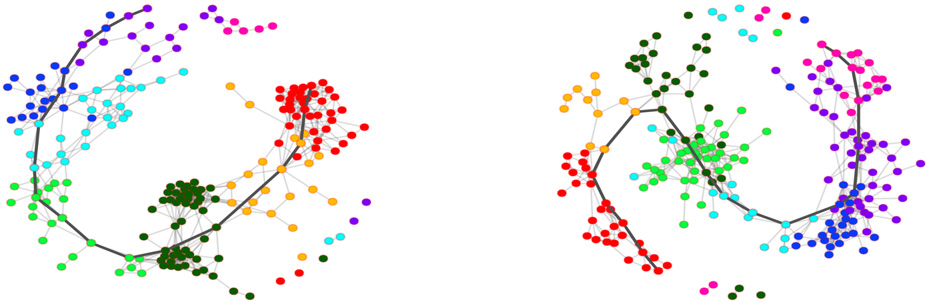
\includegraphics[width=0.9\textwidth]{fig/sociopatterns.jpg}
  \caption[Aggregated networks for two different days of the
  SocioPatterns dataset.]{Aggregated networks for two different days
    of the SocioPatterns dataset. Nodes are colored from red to purple
    according to their arrival
    time. (Source:~\cite{isella_whats_2011}.)}%
  \label{fig:sp_plot}
\end{figure}

The interactions times of the SocioPatterns dataset show that there
are limited interactions between visitors entering the exhibition more
than one hour apart (see~\autoref{fig:sp_plot}). A consequence of this
is that the network diameter of the daily aggregated graphs connects
visitors entering the venue at successive times, as can be seen in the
figure.

Another interesting properties of these interactions is their
lengths. Most of the interaction last less than one minute, as can be
expected in the context of visitors in a museum exhibition. The
distribution of the interaction durations shows broad tails, decaying
slightly faster than a power law~\cite{isella_whats_2011}.

The temporal network has also been used in a variety of contexts from
percolation analysis and dynamical spreading to community
detection~\cite{isella_whats_2011}. These studies have confirmed that
topological criteria detect efficiently the edges acting as bridges
between communities~\cite{girvan_community_2002, holme_attack_2002}.

Many empirical temporal networks exhibit periodic
patterns~\cite{holme_modern_2015}. Many papers have explored
traditional network statistics and methods to uncover cyclic behaviour
in various datasets, mainly telecommunication
networks~\cite{jo_circadian_2012, aledavood_daily_2015,
  holme_network_2003, aledavood_digital_2015}.

Visualizations show significant variations in the patterns of the
daily aggregated graphs between weekdays and weekends (see the
SocioPatterns poster in appendix). This project will attempt to apply
the topological methods on an empirical dataset to try to detect
periodicity.

\section{Computational environment}%
\label{sec:comp-envir}

The analysis pipeline described in~\autoref{sec:analysis-pipeline} is
entirely implemented in Python. For these tests, we use Python~3.5,
with Numpy~1.15.1. The library
Dionysus~2.0.7~\cite{morozov_dionysus:_2018} is used for persistent
homology, zigzag persistence, and bottleneck distance. Networks are
handled by igraph~0.7.1, and machine-learning algorithms are provided
by Scikit-Learn~0.19.2~\cite{pedregosa_scikit-learn:_2011}.

The program runs on a shared-memory system with 32 cores of 3.6~GHz,
756~GB of RAM, and 1.6~TB of storage. It runs Ubuntu Linux
16.04.5. Dionysus was compiled from the latest development version
using GCC 5.4.0 with the optimization level -O3.

\section{Results}%
\label{sec:results}

\subsection{Generative model}%
\label{sec:generative-model}

For this study, random networks have been generated with the following
parameters (keeping the notations
from~\autoref{sec:gener-model-peri}):
\begin{itemize}
\item the base graph $G$ is an Erdős-Rényi graph with 40 nodes and an
  edge probability of 90\%,
\item the total time range $T$ for the sequence of times is 200,
\item the frequency $f$ is 15/200.
\end{itemize}

\autoref{fig:density} shows the density and sample times for a single
edge. A series of presence times like this is generated for each edge
in the base graph.

\begin{figure}[ht]
  \centering
  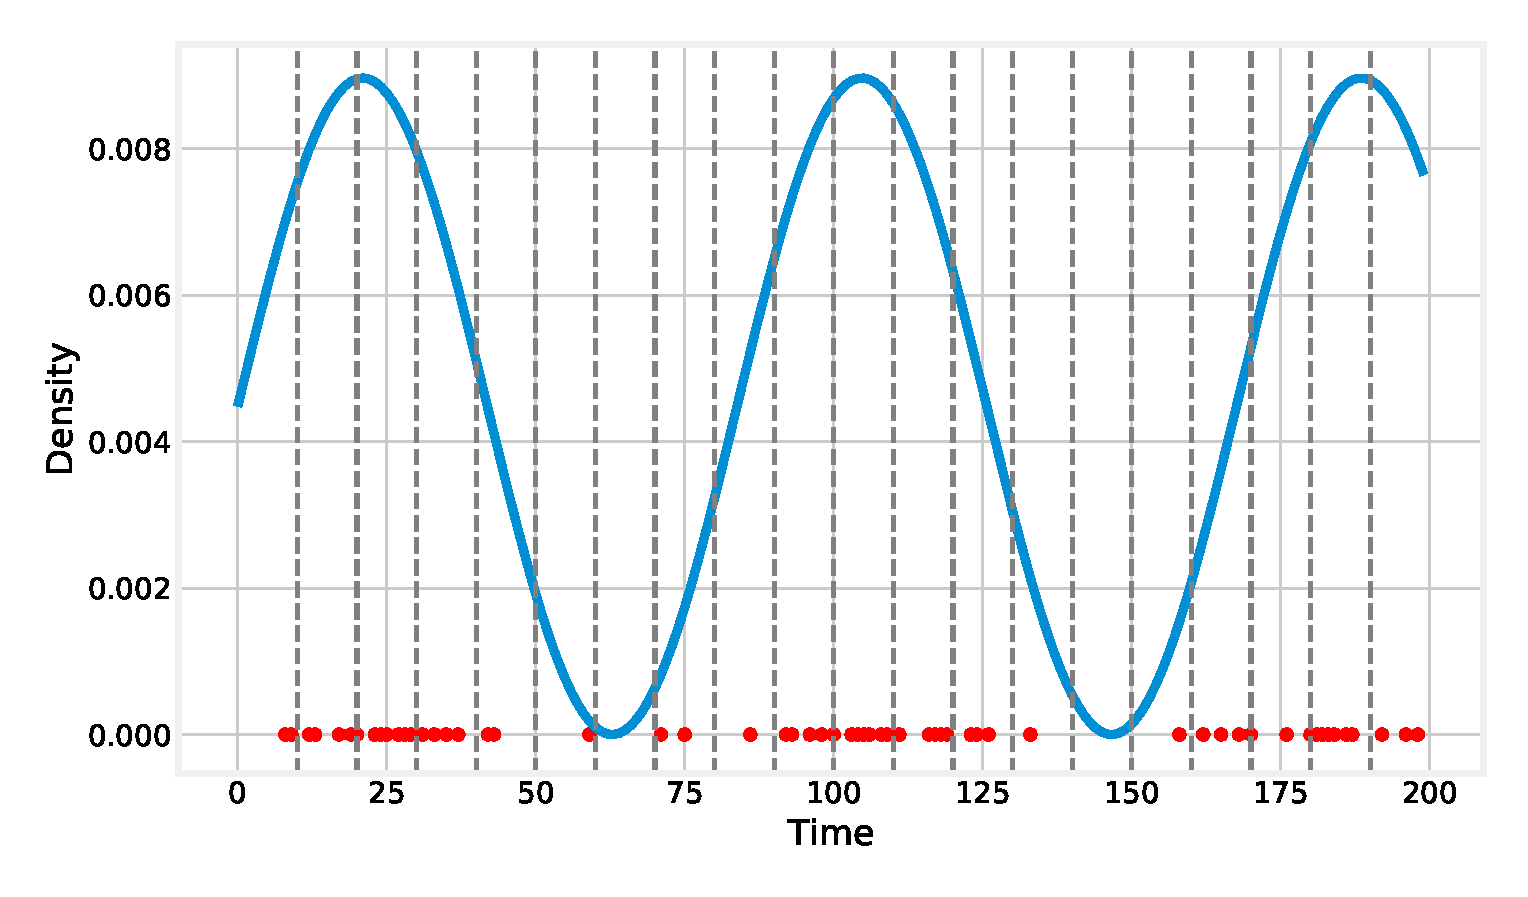
\includegraphics[width=.85\linewidth]{fig/density.pdf}
  \caption[Example of periodic density for edge times
  generation.]{Example of periodic density for edge times generation
    (blue), with random edge times (red), and the sliding windows
    (grey).}%
  \label{fig:density}
\end{figure}

The generated temporal network is then subdivided into 20
subnetworks. The sliding windows are also represented
on~\autoref{fig:density}.

From these subnetworks, persistence is computed, in the form of
persistence diagrams. An example can be found
in~\autoref{fig:diagram}.

\begin{figure}[ht]
  \centering
  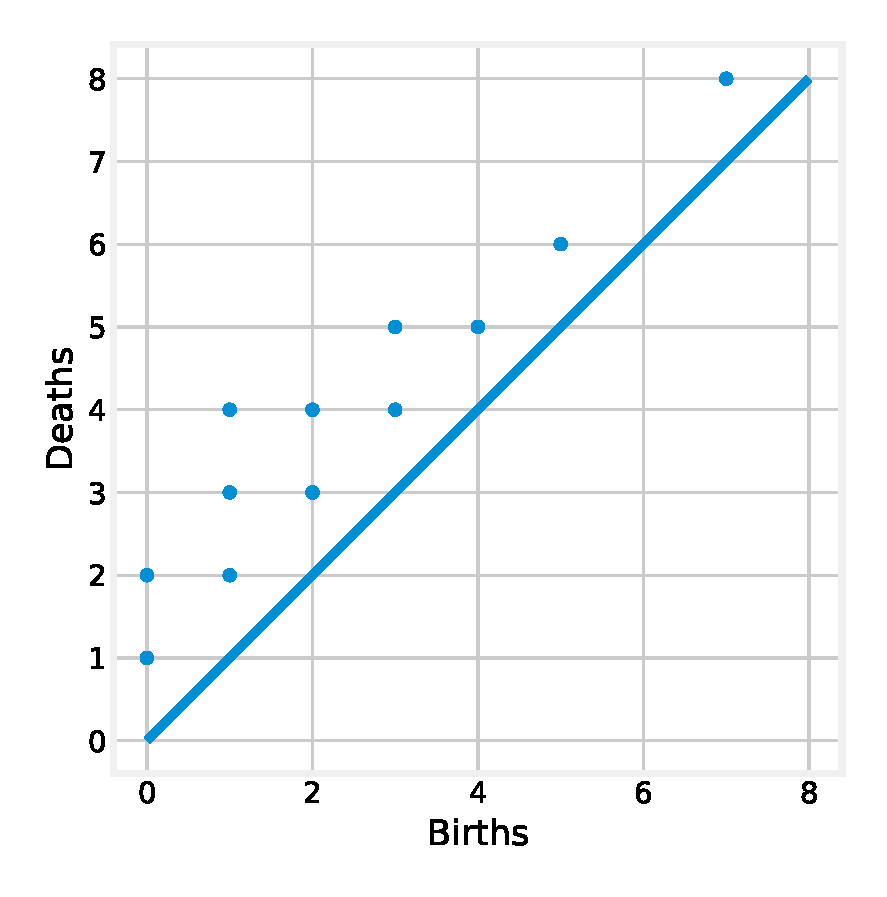
\includegraphics[width=.5\linewidth]{fig/diagram.pdf}
  \caption{Example persistence diagram.}%
  \label{fig:diagram}
\end{figure}

\autoref{fig:gen} represents the output of hierarchical clustering for
a random network, with zigzag and WRCF persistence, and the sliced
Wasserstein kernel and the bottleneck distance. This clustering is
representative of what is obtained by applying the same pipelines to
many temporal networks generated by the random model
of~\autoref{sec:gener-model-peri}.
 
\begin{figure}[ht]
  \centering
  \begin{subfigure}[b]{0.46\linewidth}
    \centering
    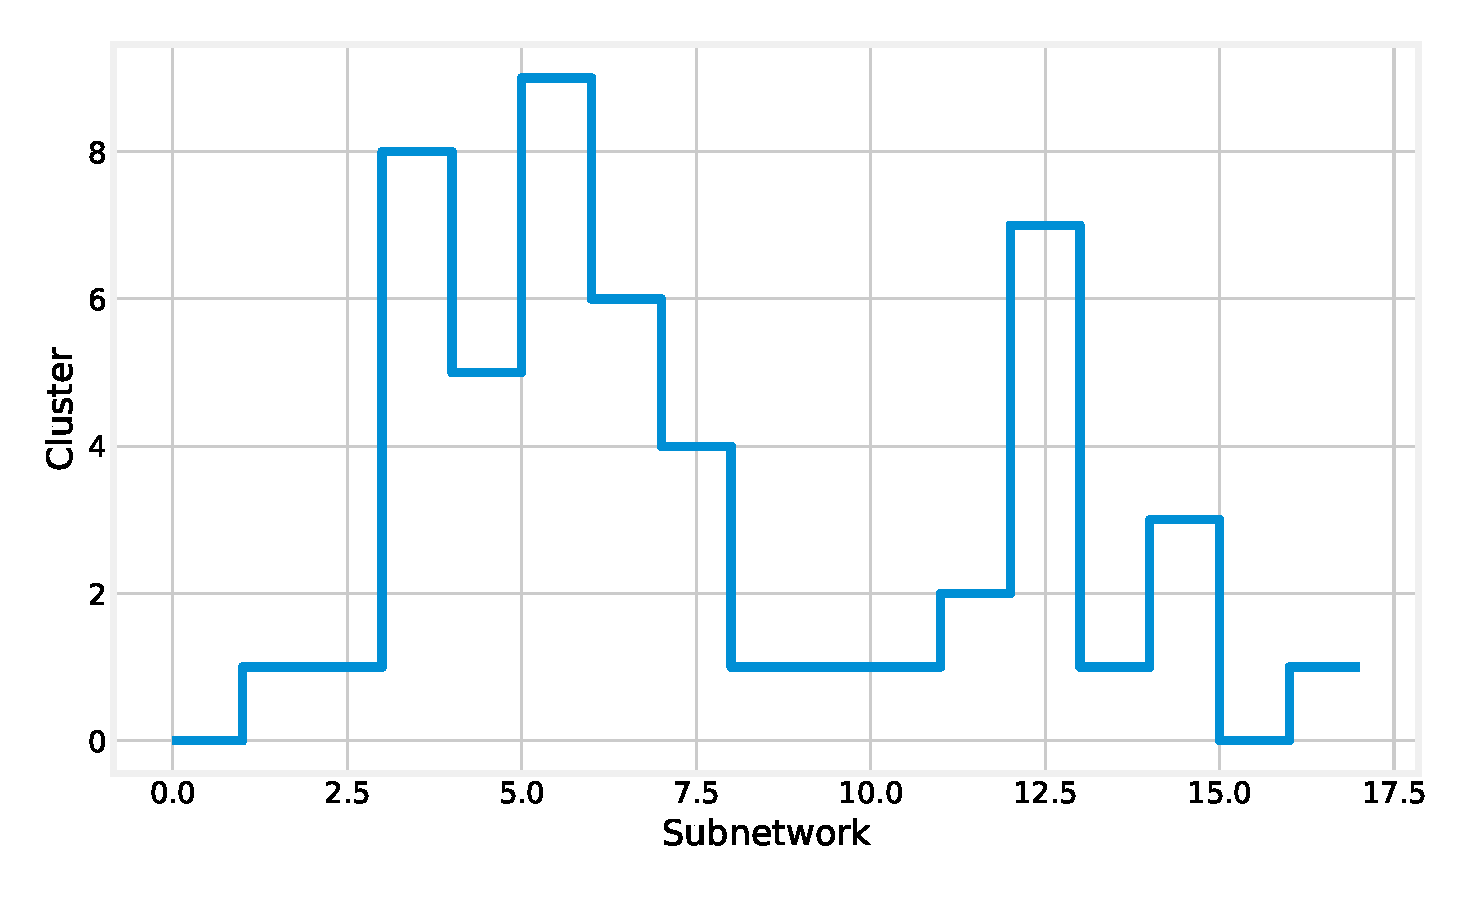
\includegraphics[width=\linewidth]{fig/gen_zz_k.pdf}
    \caption{Zigzag persistence, sliced Wasserstein kernel}%
    \label{fig:gen_zz_k}
  \end{subfigure}\qquad
  \begin{subfigure}[b]{0.46\linewidth}
    \centering
    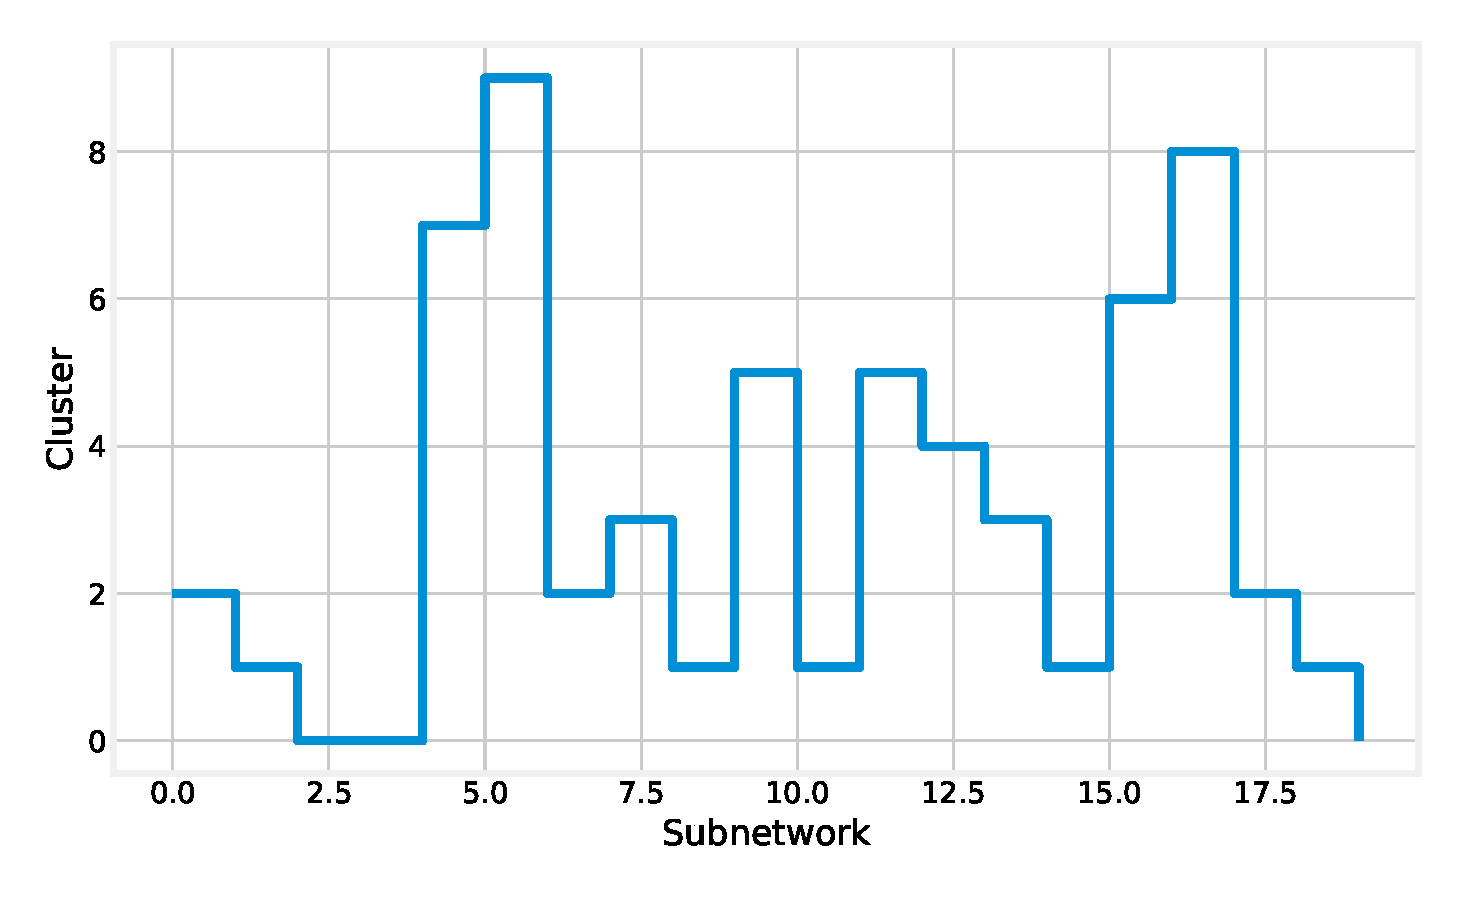
\includegraphics[width=\linewidth]{fig/gen_wrcf_k.pdf}
    \caption{WRCF, sliced Wasserstein kernel}%
    \label{fig:gen_wrcf_k}
  \end{subfigure}

  \begin{subfigure}[b]{0.46\linewidth}
    \centering
    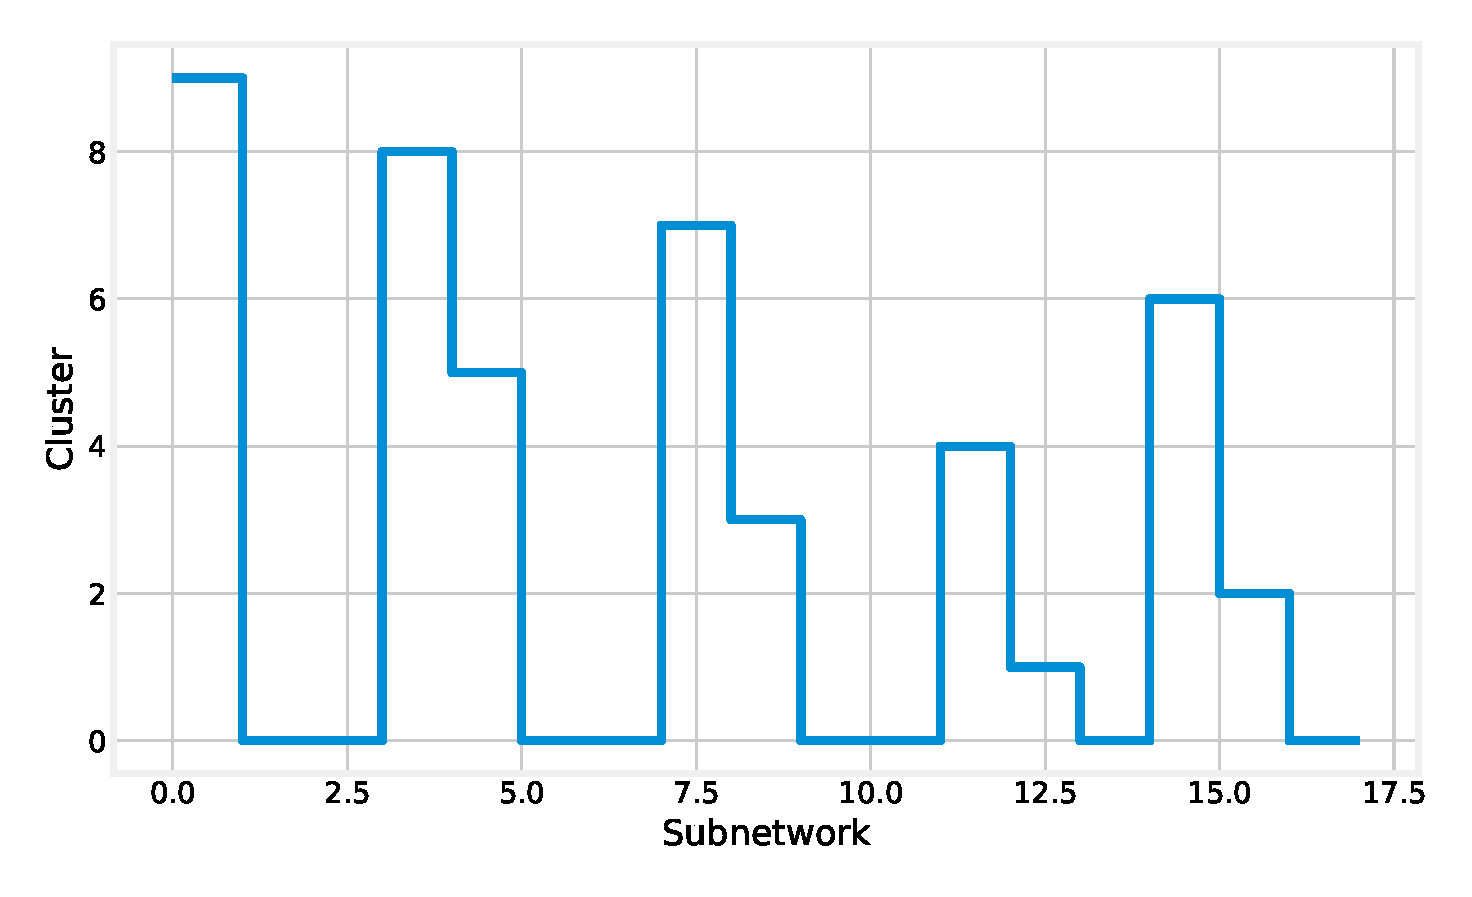
\includegraphics[width=\linewidth]{fig/gen_zz_b.pdf}
    \caption{Zigzag persistence, bottleneck distance}%
    \label{fig:gen_zz_b}
  \end{subfigure}\qquad
  \begin{subfigure}[b]{0.46\linewidth}
    \centering
    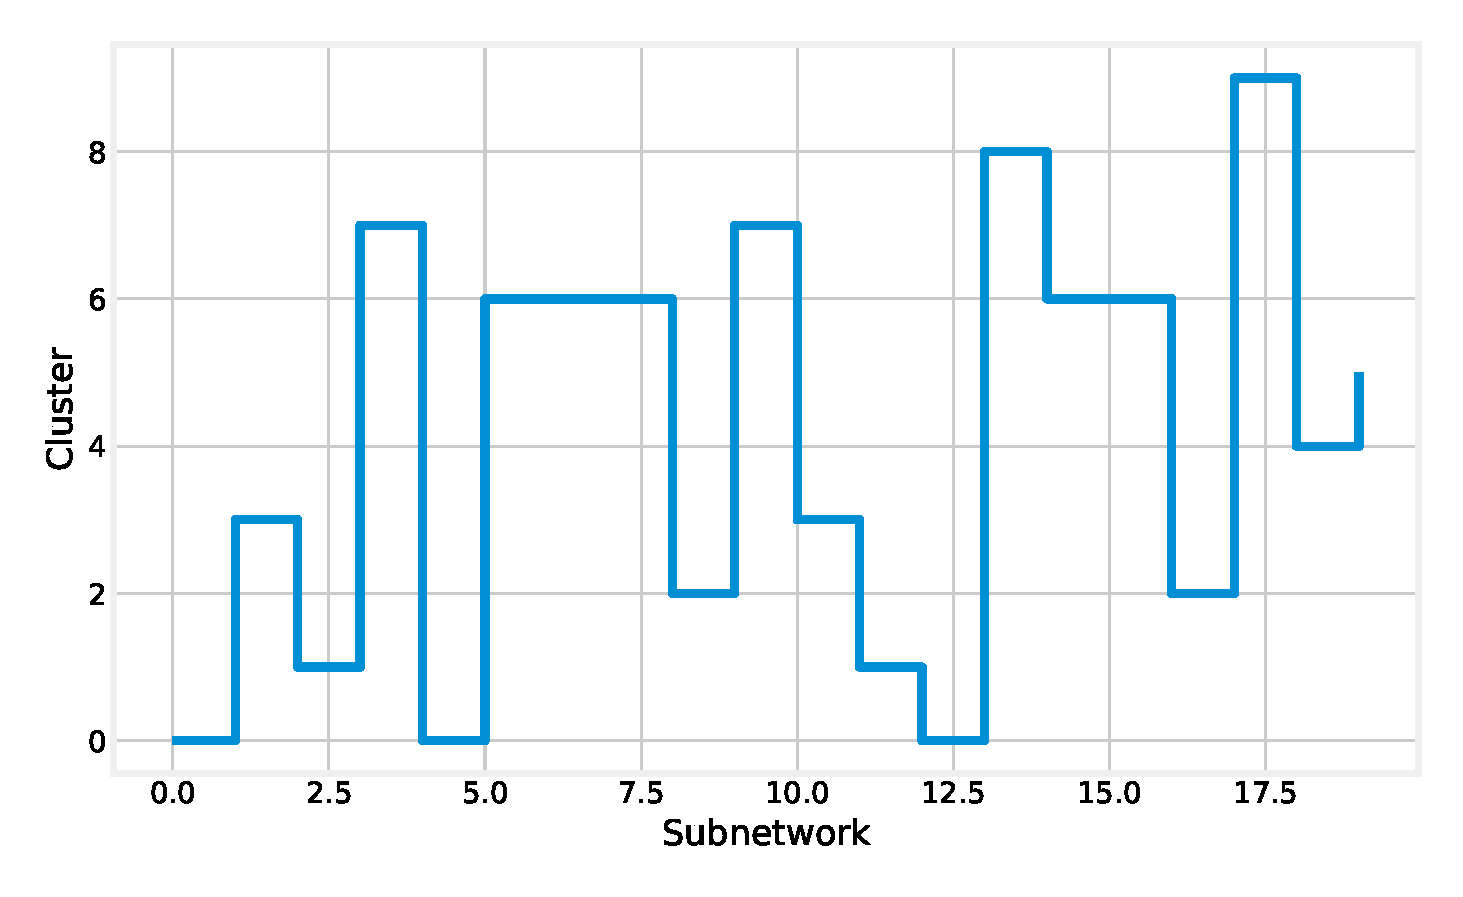
\includegraphics[width=\linewidth]{fig/gen_wrcf_b.pdf}
    \caption{WRCF, bottleneck distance}%
    \label{fig:gen_wrcf_b}
  \end{subfigure}
  \caption{Hierarchical clustering with 10 clusters of a random
    temporal network.}%
  \label{fig:gen}
\end{figure}

As we can see on the figure, the hierarchical clustering algorithm is
able to determine the periodicity of the temporal networks when using
the sliced Wasserstein kernel. However, with the simple bottleneck
distance, the periodicity is not correctly detected. The periodicity
detection can be confirmed by moving further up in the dendrogram of
the clustering algorithm. With only 2 or 3 clusters, the low and high
sections of the density (\autoref{fig:density}) are still accurately
classified with the sliced Wasserstein kernel, while the subnetworks
are distributed randomly among the clusters with the bottleneck
distance.

Somewhat less clear is the comparison between zigzag persistence and
WRCF persistence. When generating many samples from the random
temporal network model, WRCF and sliced Wasserstein kernel clustering
is noisier and less consistent in its periodicity detection than its
zigzag persistence counterpart. This indicates that the aggregation of
the temporal subnetworks lead to the creation of artificial
topological features that introduce noise in the
dataset. (See~\autoref{sec:zigzag-persistence-1} for details on why
aggregation introduce artificial simplices in the temporal network.)

\subsection{SocioPatterns dataset}%
\label{sec:soci-datas}

\begin{figure}[ht]
  \centering
  \begin{subfigure}[b]{0.8\linewidth}
  \centering
  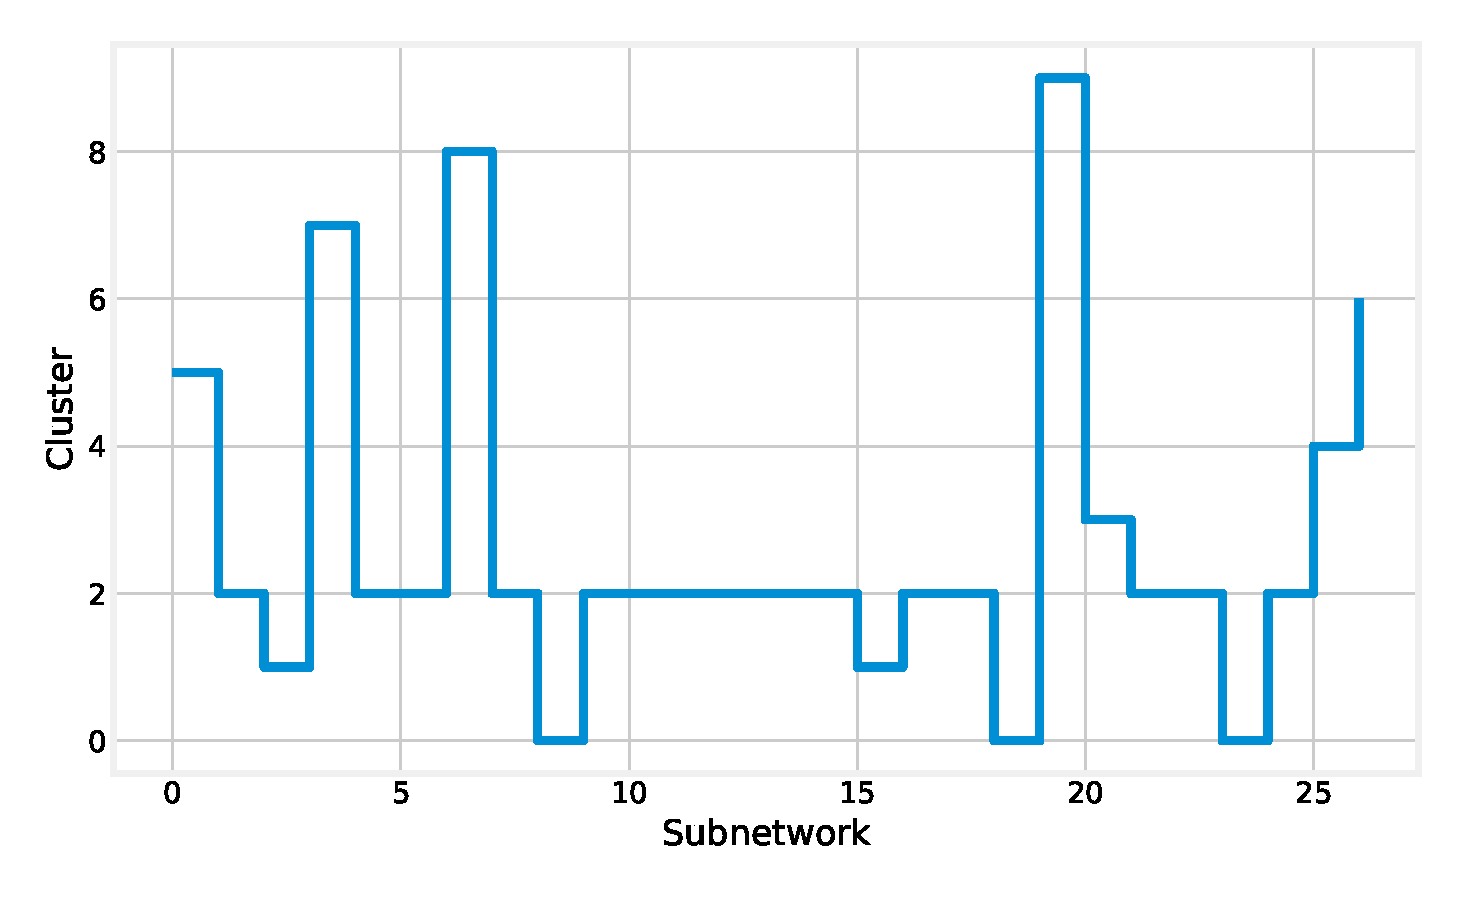
\includegraphics[width=.85\linewidth]{fig/sp_zz_k.pdf}
  \caption{Zigzag persistence, sliced Wasserstein kernel}%
  \label{fig:sp_zz_k}
\end{subfigure}
\begin{subfigure}[b]{0.8\linewidth}
  \centering
  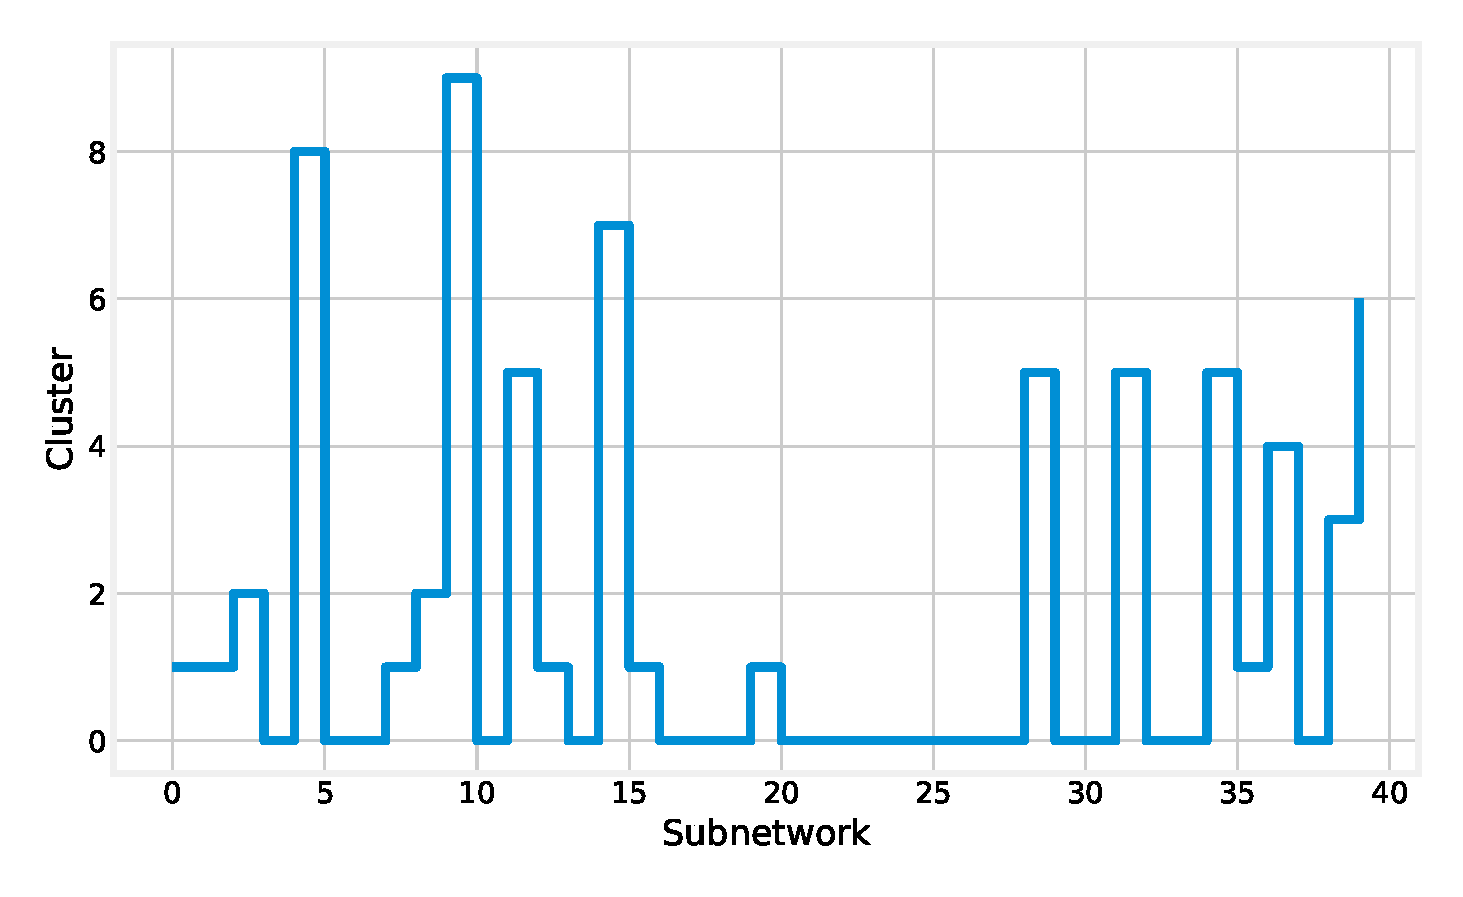
\includegraphics[width=.85\linewidth]{fig/sp_wrcf_k.pdf}
  \caption{WRCF, sliced Wasserstein kernel}%
  \label{fig:sp_wrcf_k}
\end{subfigure}
\caption{Hierarchical clustering with 10 clusters of the SocioPatterns
  dataset.}%
\label{fig:sp}
\end{figure}

In the study of the SocioPatterns dataset, we expect to uncover a
periodicity on a scale of a day. Therefore, we would like to partition
the time range of the dataset into windows approximately the length of
a day. However, this leads to very sparse subnetworks, which do not
exhibit enough topological features for a complete study. Since the
main periodicity in the dataset is expected to be a weekday/weekend
succession, we choose a resolution of two days.

The previous section has demonstrated that the sliced Wasserstein
kernel was the most suitable to uncover periodicity in a temporal
network. The results, with zigzag persistence and WRCF, of the
hierarchical clustering algorithm are shown in~\autoref{fig:sp}.

\begin{figure}[ht]
  \centering
  \begin{subfigure}[b]{0.45\linewidth}
    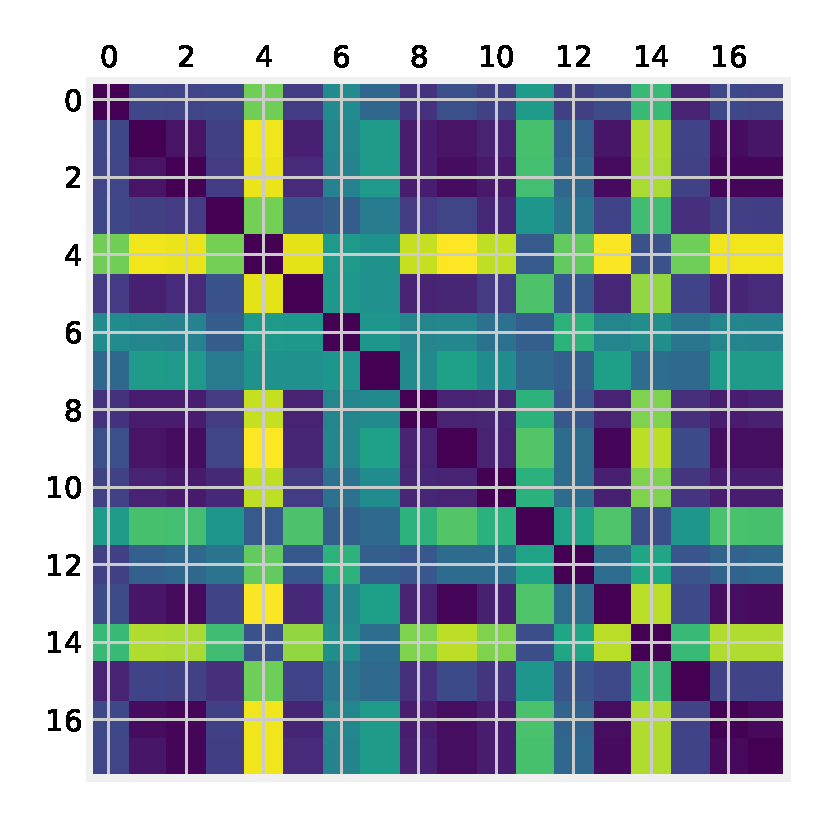
\includegraphics[width=\linewidth]{fig/gen_zz_gram1.pdf}
    \caption{Generative model}%
    \label{fig:gram_gen}
  \end{subfigure}\qquad
  \begin{subfigure}[b]{0.45\linewidth}
    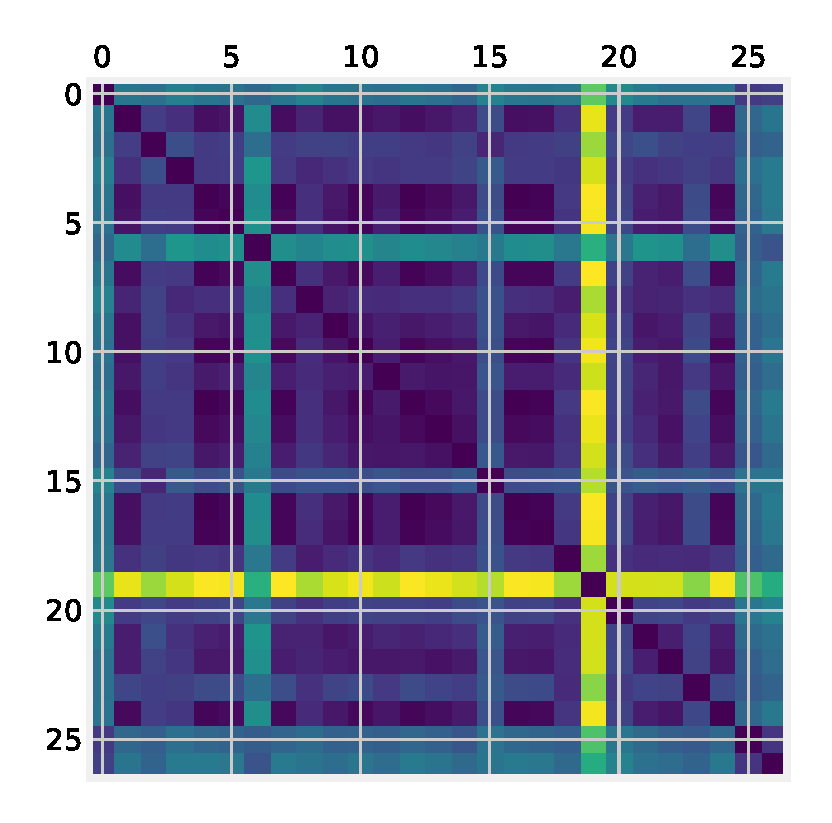
\includegraphics[width=\linewidth]{fig/sp_zz_gram1.pdf}
    \caption{SocioPatterns dataset}%
    \label{fig:gram_sp}
  \end{subfigure}
  \caption{Gram matrices of the sliced Wasserstein kernel with zigzag
    persistence.}%
  \label{fig:gram}
\end{figure}

However, the subnetworks do not cluster periodically in either
case. This is confirmed by visualizing the Gram matrix of the sliced
Wasserstein kernel (\autoref{fig:gram}). The Gram matrix obtained with
the generative model exhibit a cyclical pattern, while the one from
the SocioPatterns dataset do not show enough distinctions between the
subnetworks.

It is unclear whether this is due to the analysis pipeline, or to the
temporal network itself not exhibiting enough periodicity on a
topological level. To confirm this, one would need to compare our
analysis with one using traditional network statistics, such as the
ones in~\cite{jo_circadian_2012, aledavood_daily_2015,
  holme_network_2003, aledavood_digital_2015}. Other empirical
networks, such as telecommunication networks, may also exhibit more
obvious cyclical patterns, where topological features might be useful.

\chapter{Conclusions}%
\label{cha:conclusions}

\section{Topological data analysis of temporal networks}%
\label{sec:topol-data-analys}

Periodicity detection on our generative model has proven
successful. More importantly, topological features and persistent
homology seem to play an important part in the classification
task. The general idea of partitioning the time range of a temporal
network into sliding windows, and running an unsupervised clustering
algorithm, works in the context of periodicity detection.

More generally, we have introduced persistent homology and topological
data analysis methods for the study of temporal networks. Building on
previous work clustering different temporal network generative models
with persistent homology~\cite{price-wright_topological_2015}, we have
expanded both the methods used and the applications, solving the
real-world problem of periodicity detection. All in all, it is clear
that persistent homology is a promising new direction for the study of
temporal networks.

Topological data analysis is a recent field, with new methods and
approaches being constantly developed and improved. In this project,
we have compared different approaches. In the context of periodicity
detection, zigzag persistence is a small improvement over the
topological analysis of aggregated graphs using weight rank clique
filtration. If this result was confirmed by other studies, it would be
an interesting development, as it would imply that the temporal aspect
is essential and cannot be discarded easily when studying temporal
networks.

One of the most active research areas of topological data analysis has
been its applications in machine learning. Considerable efforts have
been deployed in the development of various vectorization techniques
to embed topological information into a feature space suitable for
statistical learning algorithms. In this project, a few of these
methods have been compared for their theoretical guarantees, and their
practical applications in periodicity detection. From a mathematical
point of view, kernels seem the most promising approach, by offering
strong stability properties and algebraic structures on the feature
space. This development leads to a broader class of applications in
machine learning where topological analysis can be useful. These
theoretical advances have translated into much better results for
periodicity detection. The simple bottleneck distance in the space of
diagram (with a structure of metric space) was not able to determine
any kind of periodicity in the random networks, whereas the sliced
Wasserstein kernel (embedding persistence diagrams in its RKHS, with
an metric equivalent to the distance in the space of persistence
diagrams) picked up the period accurately. This confirms previous work
on shape classification, where kernels on persistence diagrams
significantly outperformed other feature
embeddings~\cite{kusano_kernel_2017, reininghaus_stable_2015,
  carriere_sliced_2017}.

Finally, we have tried to apply the same analysis to detect
periodicity on real-world data, the SocioPatterns dataset. Our model
was not able to detect a periodicity with a change of patterns between
the weekdays and the weekends. This is unclear whether it is due to
the limits in some part of our analysis pipeline, or to the
periodicity in the network being non-topological in nature. A future
study might focus on combining topological features with traditional
network statistics.

\section{Future work}%
\label{sec:future-work}

Further study of topological features of temporal networks is
needed. We could imagine other applications than periodicity
detection, such as community
detection~\cite{girvan_community_2002}. Many standard methods are
difficult to adapt to temporal network models, and computational
topology could bring an additional perspective in these tasks, by
complementing traditional network statistics.

In the specific context of periodicity detection, this analysis can be
expanded by varying the parameters such as the resolution and the
overlap. It could be especially useful for inferring the period in a
temporal network.

One should also explore the other vectorization methods in the context
of periodicity detection. It would be interesting to know how
persistence images, or the other kernels, perform in this task. Last
but not least, it is essential to compare the performance of the
topological features with more traditional network statistics. It
would also be interesting to combine both aspects and use both set of
features in machine-learning tasks.

Finally, temporal networks seem to be the ideal context to apply
multidimensional persistence. For instance, the weight rank clique
filtration adds a ``weight'' dimension to the existing time
dimension. In theory, it would be possible to use this by constructing
a 2-parameter filtration on the network, and computing persistence on
it.




\appendix

\chapter{Topology}%
\label{cha:topology}

In the following chapter, we recall a few essential definitions in
topology. This is in large part taken from~\cite{golse_mat321_2015}.

In this chapter, all vector spaces will be over a field $\mathbb{K}$,
which is either the field of real numbers $\mathbb{R}$ or the field of
complex numbers $\mathbb{C}$.

\section{Metric spaces}%
\label{sec:metric-spaces}

\begin{defn}[Distance, metric space]
  An application $d : X \times X \mapsto \mathbb{R}^+$ is a \emph{distance}
  over $X$ if
  \begin{enumerate}[(i)]
  \item $\forall x,y\in X,\; d(x,y) = 0 \Leftrightarrow x=y$ (separation),
  \item $\forall x,y\in X,\; d(x,y) = d(y,x)$ (symmetry),
  \item $\forall x,y,z\in X,\; d(x,y) + d(y,z) \geq d(x,z)$ (triangle inequality).
  \end{enumerate}

  In this case, $(X, d)$ is called a \emph{metric space}.
\end{defn}

If $Y$ is a subset of $X$ and $X$ is a metric space (with the distance
$d$), then $(Y, d)$ is immediately a metric space itself. $d_Y$ is
called the \emph{induced metric} on $Y$.

%% example?

If $(X,d)$ is metric space, then for all $x\in X$ and $r>0$, the set
\[ B(x,r) := \{y\in X : d(x,y) < r\} \] is called the \emph{open ball}
centered at $x$ and of radius $r$. The \emph{closed ball} centered at
$x$ and of radius $r$ is defined by
\[ B_c(x,r) := \{y\in X : d(x,y) \leq r\}. \]

%% example/figure?

An important class of metric spaces is the one where the set $X$ is
itself a normed vector space.

\begin{defn}[Norm]
  Let $V$ be a vector space over $\mathbb{K}$. An application
  $N: V\mapsto\mathbb{R}^+$ is a \emph{norm} over $V$ if
  \begin{enumerate}[(i)]
  \item $\forall x\in V,\; N(x) = 0 \Leftrightarrow x=0$,
  \item
    $\forall x\in V, \forall \lambda\in\mathbb{K},\; N(\lambda x) =
    \lvert\lambda\rvert N(x)$,
  \item $\forall x,y\in V,\; N(x) + N(y) \geq N(x+Y)$.
  \end{enumerate}
\end{defn}

Let $(V,N)$ be a normed vector space. For every subset $X$ of $V$, one
can define $d(x,y) := N(x-y)$ for all $x,y\in X$. Using the properties
of the norm $N$, one can check easily that $d$ is a distance, and
therefore $(X,d)$ is a metric space.

%% examples?

There are many norms possible on a vector space. This brings the need
to compare these various norms.

\begin{defn}[Norm equivalence]
  Let $V$ be a vector space. Two norms $N_1$ and $N_2$ on $V$ are said
  to be \emph{equivalent} if there are two constants $C_1$ and $C_2$
  such that
  \[ \forall x\in V,\quad N_1(x) \leq C_1 N_2(x) \quad\text{and}\quad N_2(x)
    \leq C_2 N_1(x). \]
\end{defn}

Geometrically speaking, two norms are equivalent if the unit ball for
the norm $N_1$ contains a non-empty ball centred at 0 for the norm
$N_2$, and vice-versa.

%% all norms are equivalent in a vector space of finite dimension?

\section{Completeness}%
\label{sec:completeness}

\begin{defn}[Convergence]
  A sequence ${(x_n)}_{n\in\mathbb{N}}$ of elements of a metric space
  $(X,d)$ \emph{converges} to a limit $x$ if
  \[ \lim_{n\rightarrow\infty} d(x_n,x) = 0. \]
\end{defn}

\begin{defn}[Cauchy sequence]
  A sequence ${(x_n)}_{n\in\mathbb{N}}$ of elements of a metric space
  $(X,d)$ is a \emph{Cauchy sequence} if
  \[ \forall\varepsilon>0, \exists n_0\in\mathbb{N},\; \text{such
      that:}\; \forall n,m\geq n_0,\; d(x_n, x_m) < \varepsilon. \]
\end{defn}

Note that every convergent sequence is a Cauchy sequence, but the
opposite is not true in general. %% counter-example?

\begin{defn}[Completeness]
  A metric space $(X,d)$ is \emph{complete} if, and only if, every
  Cauchy sequence converges to an element of $X$.
\end{defn}

%% examples?

%% properties? would need open/close

\begin{defn}[Banach space]
  A \emph{Banach space} is a complete normed vector space.
\end{defn}

\section{Hilbert spaces}%
\label{sec:hilbert-spaces}

In this section, vector spaces are defined over~$\mathbb{C}$. The
theory extends easily to vector spaces over~$\mathbb{R}$.

An application $L$ between two $\mathbb{C}$-vector spaces $V$ and $W$
is said to be \emph{anti-linear} if
\[ \forall \lambda,\mu\in\mathbb{C}, \forall x,y\in V,\; L(\lambda x +
  \mu y) = \bar{\lambda} L(x) + \bar{\mu} y. \]

\begin{defn}[Hermitian product]
  An application $\langle\cdot,\cdot\rangle : V \times V \mapsto \mathbb{C}$ is
  \begin{enumerate}[(i)]
  \item a \emph{sesquilinear form} if $x\mapsto\langle x,y \rangle$ is
    linear and $y\mapsto\langle x,y \rangle$ is anti-linear,
  \item a \emph{Hermitian form} if it is sesquilinear and
    $\langle x,y \rangle = \overline{\langle y,x \rangle}$ for all
    $x,y\in V$,
  \item a \emph{Hermitian product} if it is a Hermitian form positive
    definite, i.e.\ if $\langle x,x \rangle > 0$ for all $x \neq 0$.
  \end{enumerate}
\end{defn}

\begin{rem}
  In the case of vector spaces over $\mathbb{R}$, sesquilinear forms
  are simply bilinear, Hermitian forms are symmetric bilinear, and
  Hermitian products are inner products.
\end{rem}

\begin{prop}[Cauchy-Schwartz inequality]
  Let $\langle\cdot,\cdot\rangle$ be a Hermitian product over
  $V$. Then, for all $x,y\in V$,
  \[ \lvert\langle x,y \rangle\rvert \leq \sqrt{\langle x,x \rangle}
    \sqrt{\langle y,y \rangle}, \] where the two sides are equal if
  and only if $x$ and $y$ are linearly dependent.
\end{prop}

\begin{proof}
  Suppose that $x \neq 0$ and $y \neq 0$ (otherwise the proposition is
  obvious). For all $t > 0$, we compute
  \[ \langle x - ty, x - ty \rangle = \langle x,x \rangle - 2t
    \mathrm{Re}\langle x,y \rangle + t^2 \langle y,y \rangle \geq
    0. \]

  Thus, for all $t > 0$,
  \[ 2 \mathrm{Re} \langle x,y \rangle \leq \frac{1}{t}\langle x,x
    \rangle + t \langle y,y \rangle. \]

  We minimize the right-hand side by choosing
  \[ t = \sqrt{\frac{\langle x,x \rangle}{\langle y,y \rangle}}, \]
  thus
  \[ \mathrm{Re} \langle x,y \rangle \leq \sqrt{\langle x,x \rangle}
    \sqrt{\langle y,y \rangle}. \]

  The inequality follows by replacing $x$ by $e^{i\theta}x$ and using the fact that
  \[ \forall z\in\mathbb{C},\; \lvert z \rvert =
    \sup_{\theta\in\mathbb{R}} \mathrm{Re}\left(e^{i\theta} z
    \right). \]

  The equality case follows from setting
  $\langle x - ty, x - ty \rangle = 0$.
\end{proof}

If $\langle\cdot,\cdot\rangle$ is a Hermitian product over $V$, it can
be verified easily that the form
\[ \lVert\cdot\rVert : x \mapsto \sqrt{\langle x,x \rangle} \] is a
norm over $V$. The triangle inequality comes from the Cauchy-Schwartz
formula. %% proof?

\begin{defn}[Pre-Hilbert space]
  A \emph{pre-Hilbert space} is a vector space $V$ with a Hermitian
  product $\langle\cdot,\cdot\rangle$ and the associated norm
  $\lVert\cdot\rVert$. It is a metric space for the distance
  $d(x,y) := \lVert x-y \rVert$.
\end{defn}

\begin{defn}[Hilbert space]
  A pre-Hilbert space $H$ is a \emph{Hilbert space} if
  $(H, \lVert\cdot\rVert)$ is a Banach space.
\end{defn}

\addtocounter{chapter}{1}
\addcontentsline{toc}{chapter}{\protect\numberline{\thechapter} Infectious SocioPatterns poster}
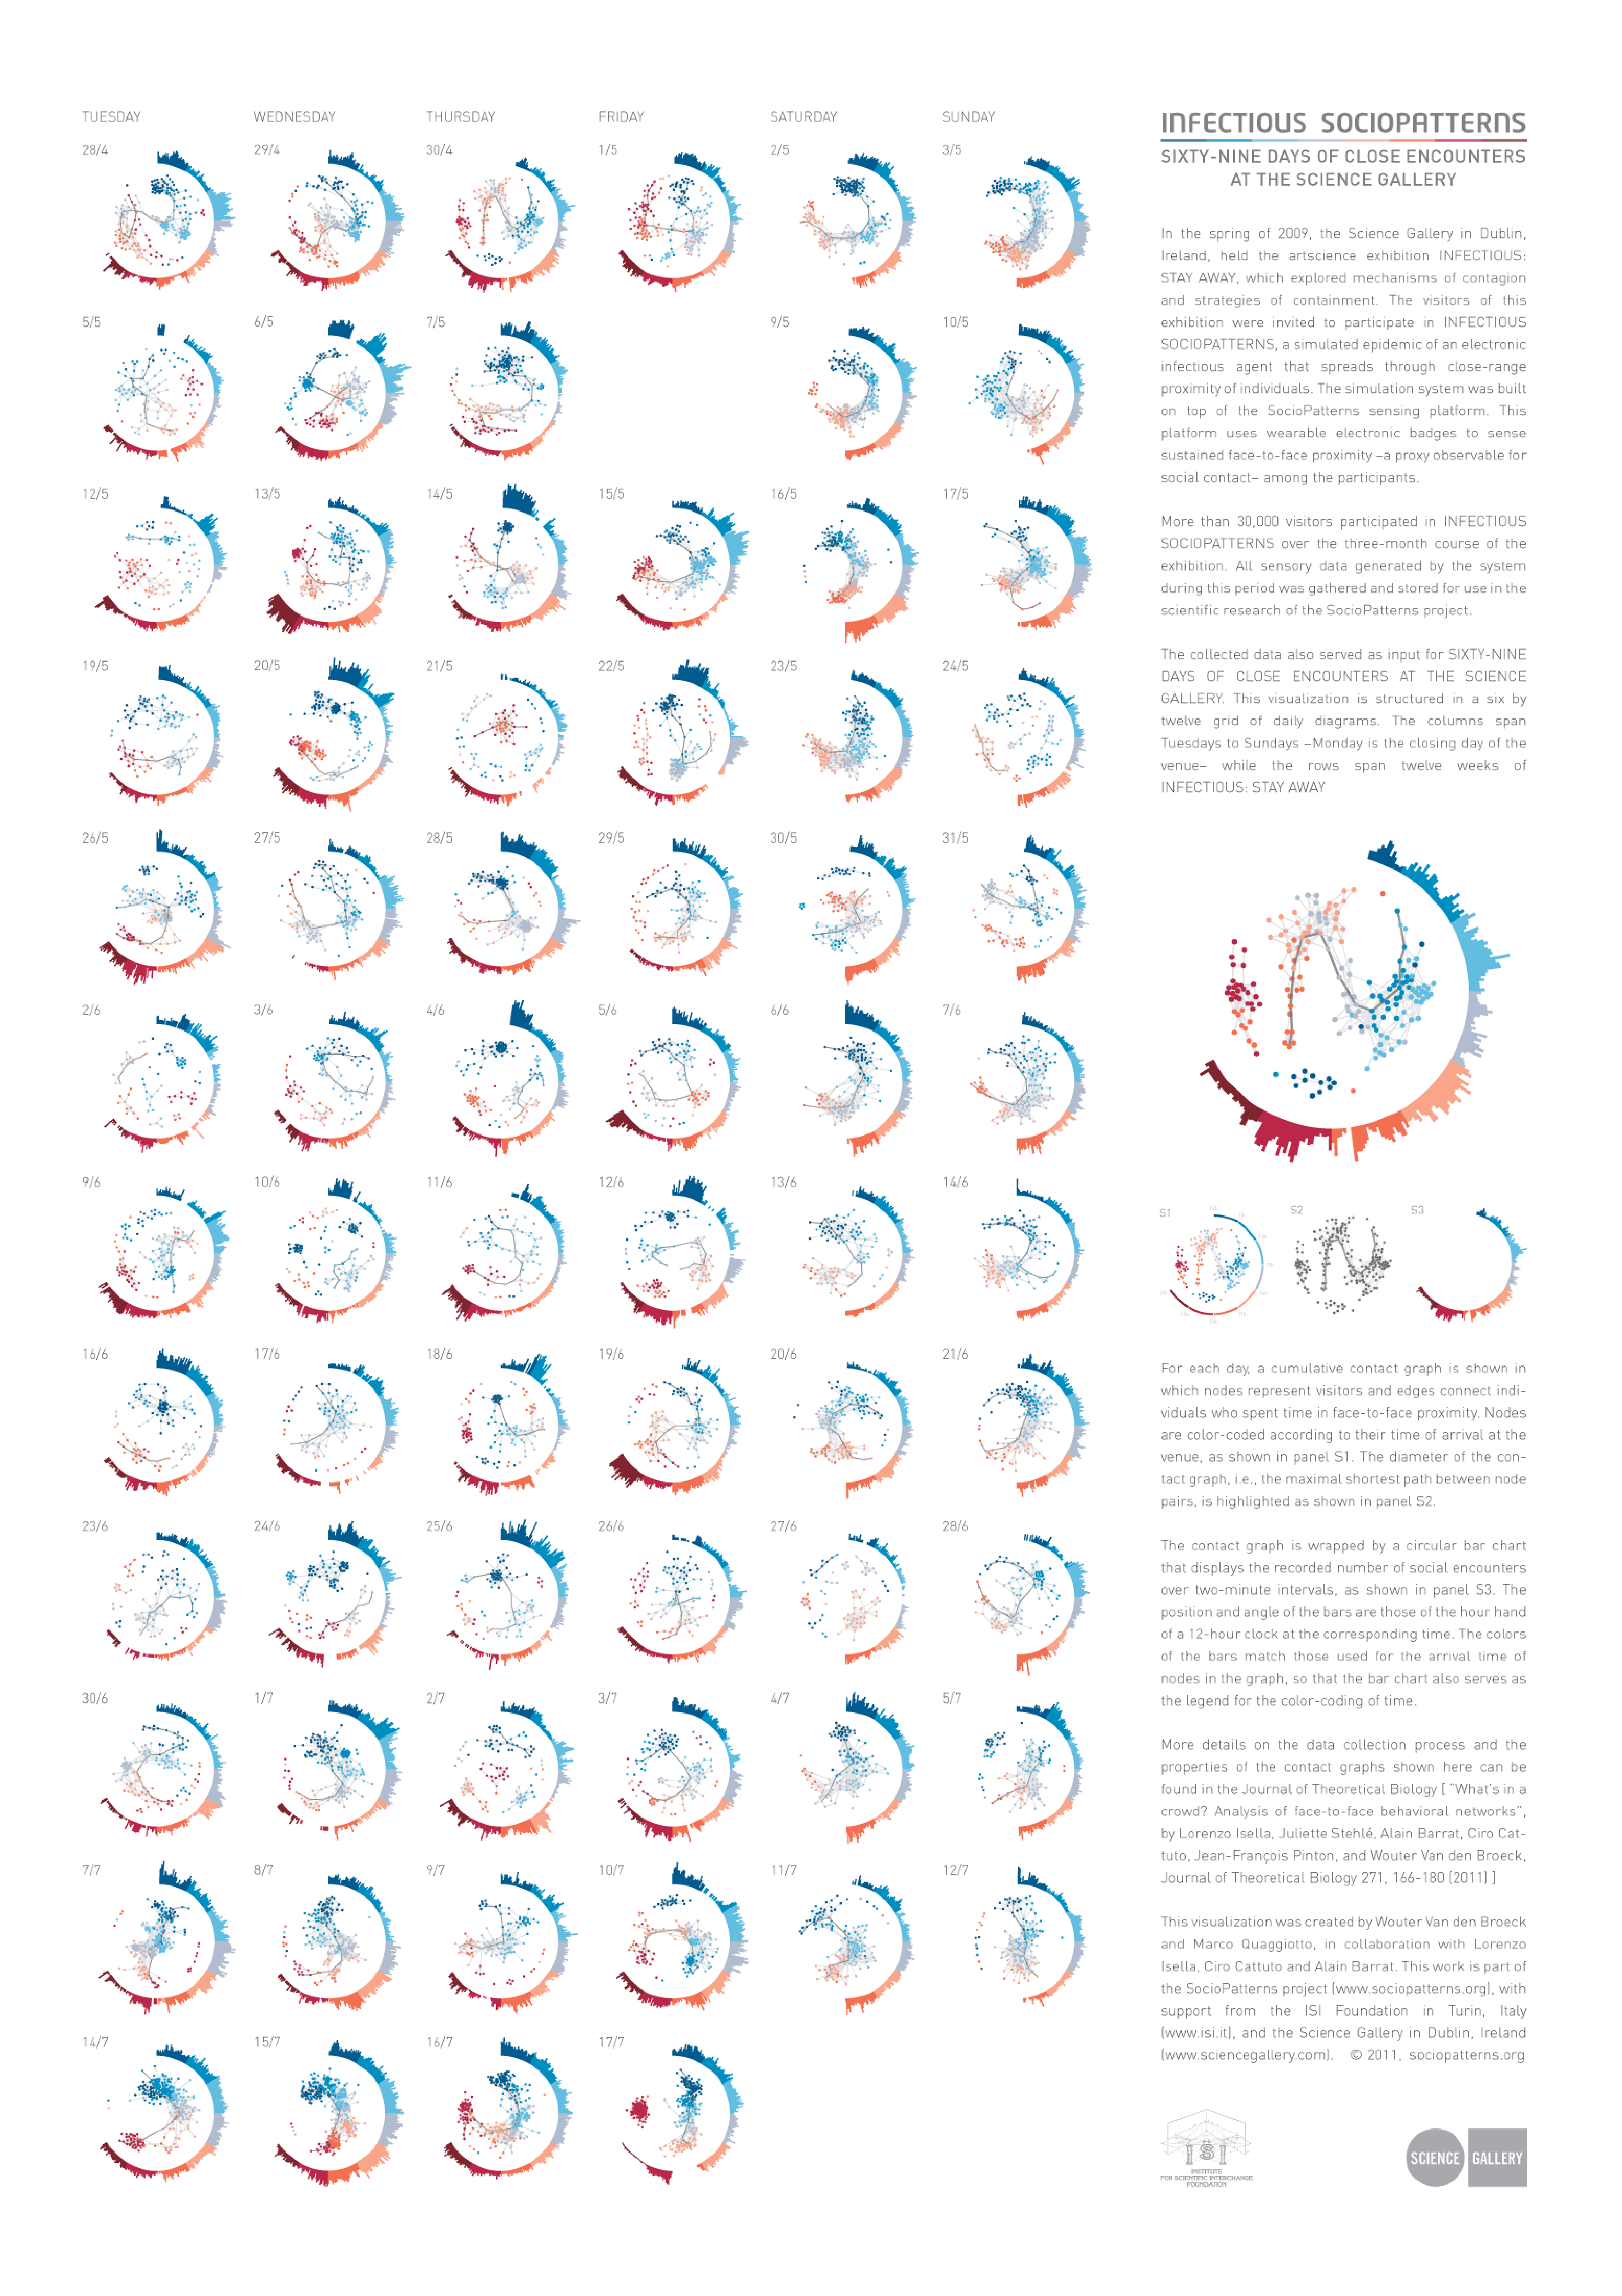
\includepdf{fig/infectious_poster.pdf}
% 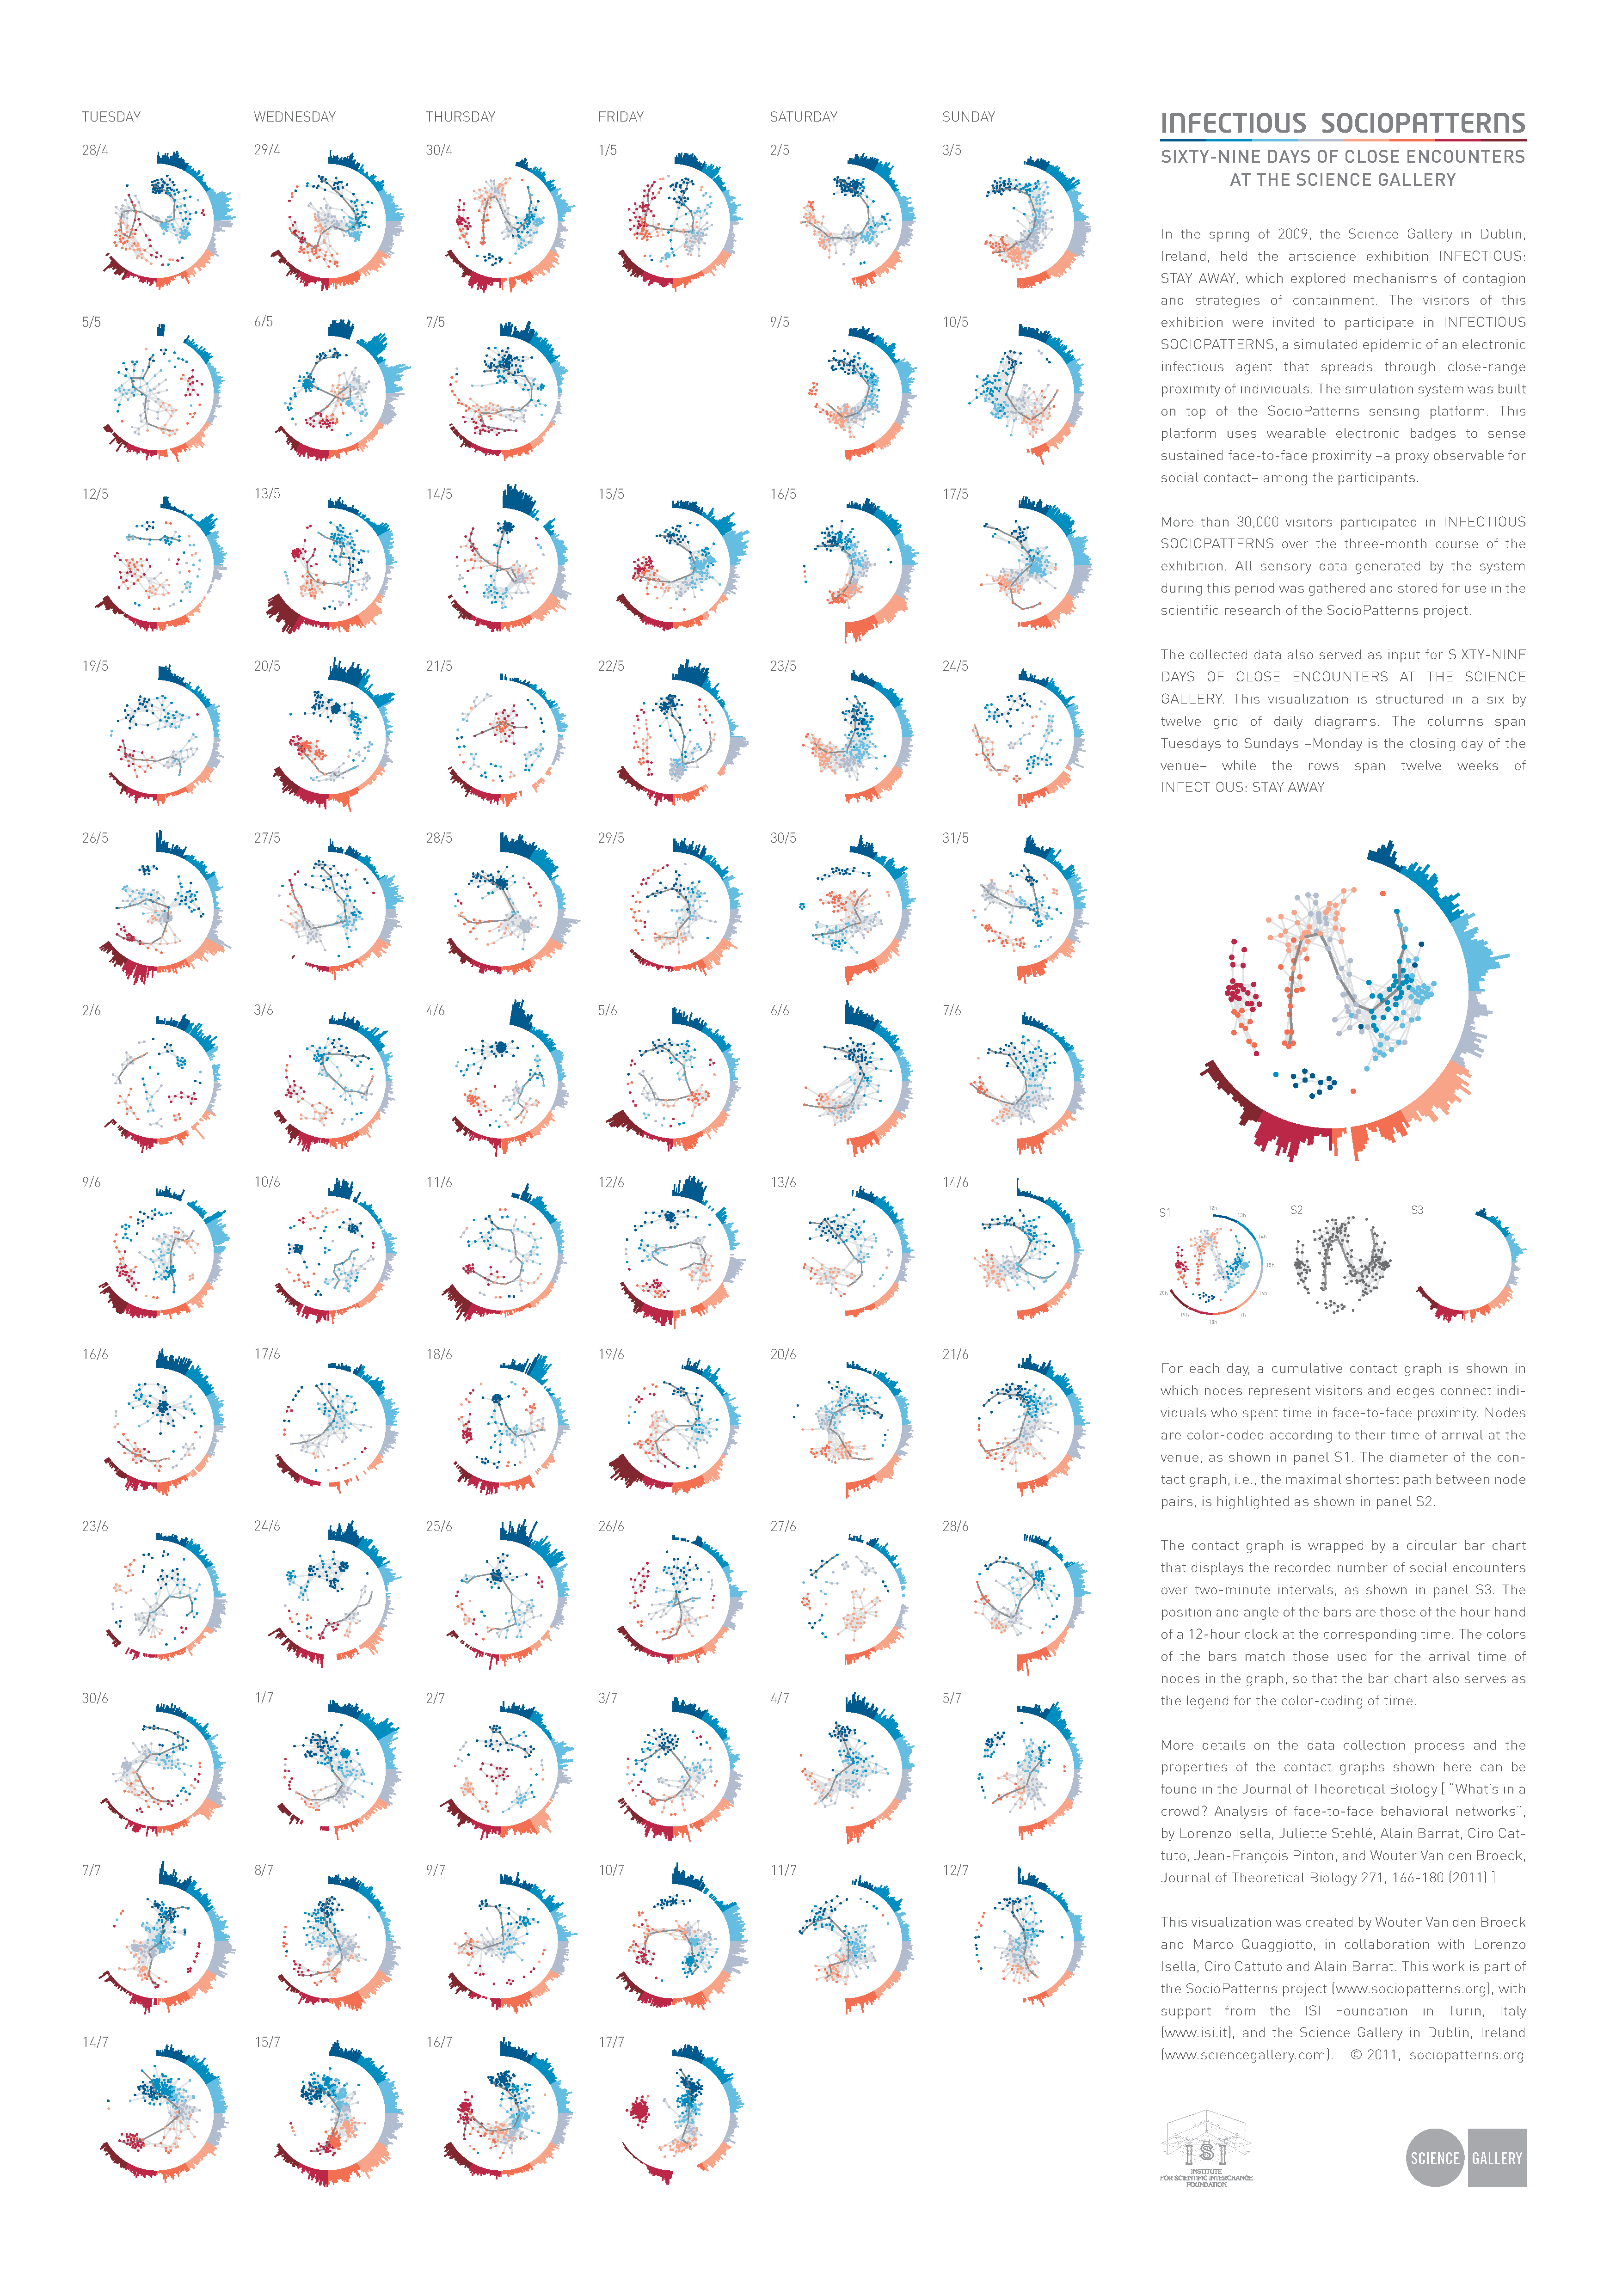
\includepdf{fig/infectious_poster_highres.pdf}\label{cha:infectious_poster}



\chapter{Code}%
\label{cha:code}

\section{\texttt{zigzag.py}}%
\label{sec:zigzagpy}

\inputminted{python}{zigzag.py}

\section{\texttt{wrcf.py}}%
\label{sec:wrcfpy}

\inputminted{python}{wrcf.py}

\section{\texttt{sliced\_wasserstein.py}}%
\label{sec:sliced_wassersteinpy}

\inputminted{python}{sliced_wasserstein.py}

\section{\texttt{generative.py}}%
\label{sec:generativepy}

\inputminted{python}{generative.py}

\section{\texttt{sociopatterns.py}}%
\label{sec:sociopatternspy}

\inputminted{python}{sociopatterns.py}

\section{\texttt{clustering.py}}%
\label{sec:clusteringpy}

\inputminted{python}{clustering.py}

\backmatter%

% \nocite{*}
\printbibliography%

\end{document}



%%% Local Variables:
%%% mode: latex
%%% TeX-master: t
%%% End:
